\chapter{The Multiple Cause Mixture Model}
\label{ch:MCMM}

\section{Introduction}
\label{sec:mcmm:intro}
Multimorph, as an unsupervised learning system, must be 
driven by an unsupervised learning algorithm, that is, 
a procedure for inducing categories from raw, unlabeled data.
%This thesis's preceding chapters have established the basic requirements for Multimorph's learning
%algorithm.
This chapter focuses on Multimorph's core learning algorithm, the Multiple Cause Mixture Model (MCMM). In particular, it motivates the choice of the MCMM \citep{saund:94}. In doing so, it explains the nature, structure, and function of MCMMs, and why an MCMM is an appropriate learning mechanism for Multimorph. 

This chapter is a culmination of the argumentation of the preceding three chapters. 
In chapters~\ref{ch:intro} and \ref{ch:lit-review}, we saw that it was precisely 
the set of \emph{nonlinear-nonsequential} models that were capable of representing 
nonconcatenative morphological structure, and that it was the properties \emph{nonlinearity}
and \emph{nonsequentiality} that give rise to this capacity. Furthermore, we in 
chapter~\ref{ch:graph} that bipartite graphs (or bipartite graphical algorithms) were a subset of NLNS algorithms. In fact, the bipartite structure of such graphs turned out to be a particularly coherent way to capture nonlinearity and nonsequentiality (REF).
%ince its relationship to the autosegmental architecture is straightforward.  
%demonstrated the equivalence between nonlinearity and 
%nonsequentiality and the mathematical properties of 
%bipartite graphs, thereby showing that bipartite graphs are 
%intrinsically nonlinear and nonsequential. It follows that bipartite graphs are 
%well-suited to represent nonconcatenative structure, and moreover, that bipartite graphical learning models are thus intrinsically well-suited to serve as learning algorithm for a ULM system. 
The present chapter homes in on a particular kind of bipartite learning algorithm, namely the MCMM. The preceding chapters provide the chain of reasoning that leads to our choice of the MCMM.

%For Multimorph, I chose a particular kind of bipartite learning model called the Multiple Cause Mixture Model (MCMM), developed by \citet{saund:94}.

%MCMMs are conducive to ULM, particularly to the UL of non-concatenative morphology, mainly because they are bipartite graphs, since it is their bipartiteness that makes them nonlinear and nonsequential. The bipartiteness of MCMMs is evident in Section~\ref{sec:architecture} (see in particular figure~\ref{fig:mcmm}), which elucidates the architecture
%of an MCMM. But while their bipartiteness is most significant for our purposes, MCMMs have other attractive properties. [which we shall discuss in this chapter.] For example, an MCMM is neither sum nor a product of experts, 

%In this chapter, therefore, we thus present a particular bipartite graphical model,  as Multimorph's core learning algorithm. In particular, I chose the bipartite graphical model known as the MCMM.
The chapter is organized as follows: Section first lays out the key components of an MCMM's structure, i.e., the attributes that all MCMMs share. Section~\ref{sec:context} then proceeds to place MCMMs in a larger of unsupervised learning algorithms, demonstrating 
%In doing so, it will break down the structure of MCMMs, demonstrating 
the similarities and differences between MCMMs and other types of learning algorithms such as Restricted Boltzmann Machines (RBM) and Latent Dirichlet Allocation (LDA). Section~\ref{sec:mixing-function} focuses a particularly important component of an MCMM, namely its \emph{mixing function}, which is a type of activation function, i.e., a function that determines the activities of nodes in neural networks.  
%Section~\ref{sec:architecture} describes the architecture of MCMMs. 
Finally, section~\ref{sec:mcmm-learning} discusses the means by which MCMMs learns, paying particular attention to Multimorph's MCMM.

%demonstrates the bipartite nature of an MCMM; compare figure~\ref{fig:mcmm} in section~\ref{sec:architecture} to the canonical bipartite structure shown in figure \ref{fig:gt-bipartite} in chapter~\ref{ch:graph}. whose bipartiteness becomes clearly evident in section~\ref{sec:architecture} Section~\ref{sec:architecture} also breaks the architecture of an MCMM, describing its basic components and how they relate to each other. hen delves deeper into the nature the MCMM, comparing and contrasting it to related learning algorithms, such as the Restricted Boltzmann Machine (RBM). Finally, section~\ref{sec:mcmm-learning} discusses the particular means by which Multimorph's MCMM learns.

% learning process itself in detail. The following section then describesSection~ fact that will become plainly evident in section~{sec:architecture}  reasoning to motivate the use of bipartite graphical learning model, specifically the MCMM, as Multimorph's algorithm.  takes this this line of argumentation to its logical conclusion i  a bipartite graphical model, namely the MCMM, tononconcatenative morphology, and thus a bipartite graphical learning algorithm is going to be at least furthermore, a bipartite archict
%In this chapter, we pre 
%From  that bipartite graphs intrinsically nonlinear and nonsequential, and that bipartite graphical learning models are 
%Thus, a bipartite architecture implies both nonlinearity and nonsequentiality and hence a capacity for representing both nonconcatenative and concatenative morphological structure. 
%
%Proposition x thus motivates the choice of bipartite graphical model to serve as Multimorph's learning suitable for learning  have the capacity to represent both nonconcatenative and concatentative morphological struThis brings us to the primary concern of the present the chapter: the choice of Multimorph's core learning algorithm. Motivated by the results of the previous chaptersparticular, the preceding chapters motivate and thus capable of representing nonconcatenative morphology. All of this is Multimorph's learning algorithm

%I chose the Multiple Cause 
%Mixture Model (MCMM) proposed by \citet{saund:94} to fill this role. The present chapter motivates this decision, and in doing so, provides a detailed exposition of the MCMM. Section~\ref{sec:architecture} first provides an overview of an MCMM's architecture, i.e., a description of its major components and the relationships between these components. Section~\ref{sec:architecture} then delves deeper into the nature the MCMM, comparing and contrasting it to related learning algorithms, such as the Restricted Boltzmann Machine (RBM).   comparing it to other including a description of their architecture in detail. describes the will be motivated in the present present chapter.  The present chapter will describe   primary objective of this chapter  motivate this decision; first of all, it will show in section~{sec:architecture}that it is a bipartite graph and thus qualifies as a nonlinear-nonsequential algorithm. \citet{saund:94}  nonlinear-nonsequential models are argued that nonlinearity and nonsequentiality were essential properties learning nonconcatenative
%morphology must be   
%Multimorph's learning algorithm is an instance of an Multiple Cause 
%Mixture Model (MCMM) proposed by \citet{saund:94}, and thus MCMMs
%is a major focus of this chapter.

%By \emph{model}, 
%we mean a set of assumptions about how the world works. Where Multimorph is concerned, 
%the ``world" is the morphology of natural languages, which, significantly, includes \emph{non-concatenative} morphology. 
%autosegmental morphology \citep{mccarthy:1981}. 
%In chapter~\ref{ch:graph}, we argued
%that in order
%for a model to be able to deal with nonconcatenative morphology,
% it must be both \textbf{nonlinear} \textbf{and}
% \textbf{nonsequential},
% i.e., satisfy both the \textsc{Nonlinearity} criterion and the \textbf{Nonsequentiality} criterion; 
% see definitions (\ref{def:nl}) and (\ref{def:ns}) and 
% proposition (\ref{prop:nlns}). We also saw in chapter~\ref{ch:graph} that these two conditions are equivalent to the two parts of the definition of biparteness. In particular, \dots.
 



% Therefore, if a model is a bipartite graphical model, then it is both nonlinear and nonsequential, which means
% that it has the capacity to model nonconcatenative morphology:
%  \begin{proposition}
%% In order for a model to be able to handle non-concatenative morphology, it must be a bipartite graph.
%% \end{proposition}
%  \label{prop:bipartite}
%If a model is a bipartite graph, it can handle nonconcatenative morphology. Moreover, if it can handle nonconcatenative morphology, it can handle concatenative morphology.
% \end{proposition}
 
%if a model is a bipartite graph, 
%it has the capacity to deal with nonconcatenative morphology.
%% of morphology are treated as the same basic phenomenon; the capacity to model nonconcatenative morphology is actually the more general capacity, since a concatenative process is essentially a nonconcatenative process with zero interdigitation. 
%That is, if there were such a thing as a ``morph discontiguity factor,'' that is, a some sort of measure of the degree to which the phonemes of different morphs tend to be interleaved (i.e., the tendency of morphs to be discontinuous), 
%%separation between phonemes of the same morpheme discontiguous the  phonemes of the same morph separated by intervening phonemes (from another morph) by those of other morphs), 
%then this metric would be zero for ``strictly concatenative'' morphological processes, and some number greater than zero for ``nonconcatenative" ones. The point is that there no categorical difference between concatenative and nonconcatenative processes. Fundamentally, the two type of processes are in fact one and the same  process.  Thus, the capacity to model noncatenative morphology implies the capacity to model concatenative morphology. 
%Noncatenative morphology can thus be regarded as the more general case.
% \begin{proposition}
%% In order for a model to be able to handle non-concatenative morphology, it must be a bipartite graph.
%% \end{proposition}
%  \label{prop:bipartite}
%If a model is a bipartite graph, it can handle nonconcatenative morphology. Moreover, if it can handle nonconcatenative morphology, it can handle concatenative morphology.
% \end{proposition}

 %call for a bipartite graph, since they are essentially equivalent to
% The Multiple Cause Mixture Model (MCMM) is a general 
% framework for unsupervised learning developed by \cite{saund:94}. 
% Section~\ref{sec:architecture} in this chapter will describe the architecture 
% of an MCMM, i.e., its key components and the relationships between these 
% components. It will become clear in this section that MCMMs are bipartite 
% graphs and thus, by proposition~\ref{prop:bipartite}, an MCMM is capable 
% of learning nonconcatenative morphology. 
 %serve as Multimorph's core learning framework.
 %  In this chapter, we shall first demonstrate an MCMM qualifies as a bipartite graph.  
%In addition to demonstrating the bipartite \emph{bona fides} of MCMMs, this chapter will, in section~\ref{sec:architecture}, discuss the architecture of an \ac{MCMM},
%i.e., is key components and the relationships between these components. 
%This chapter will also, in 
%sections~\ref{sec:mixing-function} and \ref{sec:mcmm-learning}, describe the process whereby
%an \ac{MCMM} learns. 

\section{Basic MCMM Architecture}
\label{sec:architecture}

In \citet{saund:94}, the term \emph{multiple cause mixture model} does to refer a single, 
specific algorithm, but rather to a family of algorithms, i.e., a general framework for unsupervised learning.  Since MCMMs constitute a definite category of algorithms, all MCMMs share certain key attributes. %These components and the relationships between them are the subject of this section. 
These attributes are in large part the subject of this section. 
%These are described in section~\ref{sec:architecture}. 
%so every MCMM must have certain key
%key attributes in order to qualify as an MCMM. 
%For instance, all MCMMs bipartite graphs, as illustrated in figure~\ref{fig:mcmm}. That is, for instance, 
%However, there is also room for variation among MCMMs. In particular, MCMMs may vary in their \emph{mixing function}.
%
%All MCMMs are 
%All have a the same in certain crucial ways.
%All share g There can thus be different kinds of MCMMs. 
%does not refer to a single, fully specified algorithm, but rather to a family of algorithms, 
%i.e., a \emph{framework} consisting of components that are only loosely rather fully 
%specified, thus allowing for a range of options as long as they satisfy certain criteria. 
%For example, one essential component of an MCMM is the \emph{mixing function}.


%\begin{tikzpicture}[scale=1.25]%,cap=round,>=latex]
%\coordinate [label=left:$A$] (A) at (-2cm,-1.cm);
%\coordinate [label=right:$C$] (C) at (2.2cm,-1.0cm);
%\coordinate [label=above:$B$] (B) at (1cm,1.0cm);
%\draw (A) -- node[sloped,above] {c} (B) -- node[sloped,above,] {a} (C) -- node[below] {b} (A);
%\draw[dashed] (B) -- (A-|B) ;
%\end{tikzpicture}

%\begin{figure}[ht]
%\begin{tikzpicture}
%\node[draw,circle] (A) at (90:3) {A};
%\node[draw,circle] (B) at (210:3) {B};
%\node[draw,circle] (C) at (330:3) {C};
%\draw[latex'-latex',double] (A) -- node[label=150:A-B,label=330:B-A] {} (B);
%\draw[latex'-latex',double] (A) -- node[label=30:A-C,label=210:C-A] {} (C);
%\draw[latex'-latex',double] (B) -- node[label=90:B-C,label=270:C-B] {} (C);
%\end{tikzpicture}
%\label{fig:alg-types}
%\caption{Relationship between the terms \emph{autoencoder}, \emph{MCMM}, and \emph{RBM}}
%\end{figure}

An MCMM is a graphical model consisting of two layers of nodes (or units): a \emph{surface} (or \emph{visible}) 
layer and a \emph{hidden} layer.
%of \emph{surface} or \emph{visible} units 
%and a layer of \emph{hidden} units. 
This is illustrated in figure~\ref{fig:mcmm}, where $\mathbf{m}$ 
is the vector of hidden units. The vector $\mathbf{x}_i$ is the 
original vector of surface units\footnote{Saund uses $\mathbf{d}$ 
rather than $\mathbf{x}$ to denote this vector}; it is the observed, 
real-world data. The vector $\mathbf{r}_i$ is the ``working" 
reconstruction of original data vector $\textbf{x}_i$. It is dynamic; 
it evolves as the learning process progresses, hopefully 
becoming more and more similar to $\mathbf{x}_i$. 
This is the essence of the learning process and will be 
discussed more fully in section~\ref{sec:mcmm-learning}).
that $\mathbf{x}_i$ is not directly connected to either $\mathbf{r}_i$ 
or $\mathbf{m}_i$. It is not an integrated component of the graphical 
model. Its role is to serve as a target for the reconstruction vector $\mathbf{r}_i$. 
The goal of the system as a learning model is to get $\mathbf{r}_i$ to 
match $\mathbf{x}_i$, i.e., to reconstruct $\mathbf{x}_i$ in 
$\mathbf{r}_i$ (as discussed in section~\ref{sec:mcmm-learning}).
% shall discuss this reconstruction process in more detail in section REF.

\begin{figure}[htb]
\begin{center}
%\small
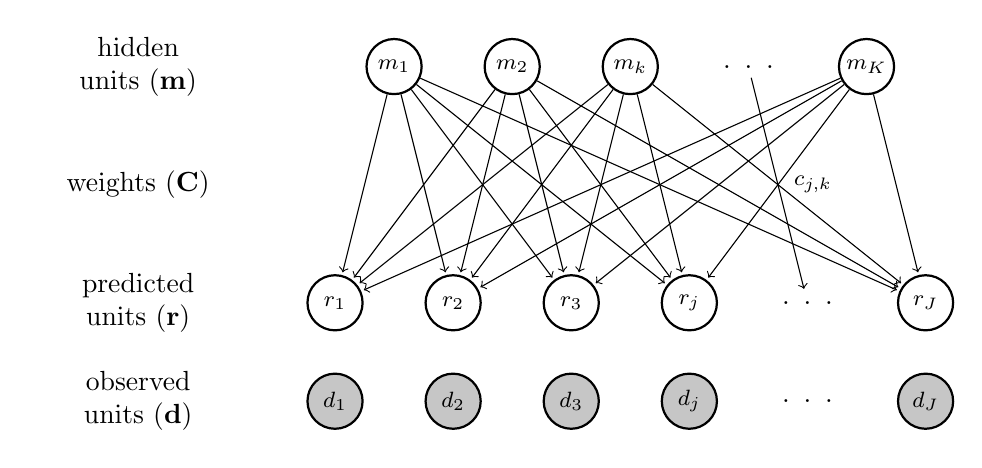
\begin{tikzpicture}[shorten >=1pt,->,draw=black!100]
	\def \rowtwoht{4.25cm}
	\def \weightlevel{2.75cm}
	\def \rowoneht{1.25cm}
	\def \basement{0cm}
	\tikzstyle{m-node}=[circle,draw=black!100,thick,inner sep=0pt,minimum size=7mm]
	\tikzstyle{r-node}=[circle,draw=black!100,thick,inner sep=0pt,minimum size=7mm]
	\tikzstyle{d-node}=[circle,draw=black!100,fill=gray!45,thick,inner sep=0pt,minimum size=7mm]
	\tikzstyle{dots}=[text width=5ex, text centered]
	\tikzstyle{annot}=[text width=17ex, text centered]
	% labels
	\node[annot] (hidden-layer) at (0cm,\rowtwoht) {hidden units ($\mathbf{m}$)};
	\node[annot] (weights) at (0cm,\weightlevel) {weights ($\mathbf{C}$)};
	\node[annot] (r-layer) at (0cm,\rowoneht) {predicted units ($\mathbf{r}$)};
	\node[annot] (d-layer) at (0cm,\basement) {observed units ($\mathbf{d}$)};
	
	\node[dots] 	(m3)	at (7.75cm,\rowtwoht)	 	{. . .};
	\node[dots] 	(r4) 	at (8.5cm,\rowoneht)   		{. . .};
	\node[dots] 	(d4) 	at (8.5cm,\basement)   		{. . .};
	
	\footnotesize
	% hidden layer
	\node[m-node] 	(m0)	at (3.25cm,\rowtwoht)		{$m_1$};
	\node[m-node] 	(m1)	at (4.75cm,\rowtwoht)		{$m_2$};
	\node[m-node] 	(m2)	at (6.25cm,\rowtwoht)	 	{$m_k$};
	\node[m-node] 	(m4)	at (9.25cm,\rowtwoht)	 	{$m_K$};
	
	% reconstructed vector
	\node[r-node] 	(r0)	at (2.5cm,\rowoneht)		{$r_1$};
	\node[r-node] 	(r1)	at (4cm,\rowoneht)		{$r_2$};
	\node[r-node] 	(r2)	at (5.5cm,\rowoneht)	 	{$r_3$};
	\node[r-node] 	(r3)	at (7cm,\rowoneht) 		{$r_j$};
	\node[r-node] 	(r5) 	at (10cm,\rowoneht)   		{$r_J$};
	%\node[r-node] 	(r6) 	at (9.75cm,\rowoneht)   	{$r_J$};
	
	% data vector
	\node[d-node] 	(d0)	at (2.5cm,\basement)		{$d_1$};
	\node[d-node] 	(d1)	at (4cm,\basement)		{$d_2$};
	\node[d-node] 	(d2)	at (5.5cm,\basement)	 	{$d_3$};
	\node[d-node] 	(d3)	at (7cm,\basement) 		{$d_j$};
	\node[d-node] 	(d5) 	at (10cm,\basement)   		{$d_J$};
	%\node[d-node] 	(d6) 	at (9.75cm,\basement)   	{$d_J$};
	
	\path 
		(m0)	edge	node	{}	(r0)
		(m0)	edge	node	{}	(r1)
		(m0)	edge	node	{}	(r2)
		(m0)	edge	node	{}	(r3)
		(m0)	edge	node	{}	(r5)
		
		(m1)	edge	node	{}	(r0)
		(m1)	edge	node	{}	(r1)
		(m1)	edge	node	{}	(r2)
		(m1)	edge	node	{}	(r3)
		(m1)	edge	node	{}	(r5)
		
		(m2)	edge	node	{}	(r0)
		(m2)	edge	node	{}	(r1)
		(m2)	edge	node	{}	(r2)
		(m2)	edge	node	{}	(r3)
		(m2)	edge	node	{}	(r5)
		(m3)	edge	node[right=1mm]	{$c_{j,k}$}	(r4)
		%	
		(m4)	edge	node	{}	(r0)
		(m4)	edge	node	{}	(r1)
		(m4)	edge	node	{}	(r2)
		(m4)	edge	node	{}	(r3)
		(m4)	edge	node	{}	(r5);
		
\end{tikzpicture}
\end{center}
\caption{Architecture of a Multiple Cause Mixture Model (MCMM)} 
\label{fig:mcmm}
\end{figure}

The vector $\mathbf{x}_i$ is but one of the $I$ rows the constitute the whole 
input corpus, the data matrix $X$. Each row contains $J$ columns. Similarly, 
$\mathbf{r}_i$, the reconstruction of $\mathbf{x}_i$, is the $i$th row in the 
$I \times J$ matrix $\mathbf{R}$. The subscript on the hidden-unit vector 
$\mathbf{m}_i$ indicates that it is related to $\mathbf{x}_i$ and $\mathbf{r}_i$. 
Each $J$ corresponds to a particular surface unit, i.e., feature. 
The hidden-unit vector is a row in the larger $I \times K$ matrix 
$\mathbf{M}$. Each of $\mathbf{M}$'s $K$ corresponds to a particular 
\emph{cluster}, and thus, the activity of each $m_{i,k}$ indicates whether the $i$th 
datapoint $\mathbf{x}_i$ (via its reconstruction $\mathbf{r}_i$) is a member of the 
$k$th cluster.  columns contains $I$, each the particular vector of hidden causes for 
the $i$th surface vector. $\mathbf{}$ has $K$ columns.

% is compared. 
%
%the vector of surface units; however, t
%The vector $\mathbf{x}_i$ is the original data vector, i.e., the original surface units
%
%Saund describes the hidden units in
%$\mathbf{m}_i$ as \textit{causes}; that is, the hidden units in an MCMM are presumed to hidden causes behind the particular arrangement of \textsc{on} and \textsc{off}) units in the original data vector $\mathbf{x}_i$. 
%
%\textsc{on} surface vectors
The hidden units are connected to surface units by a matrix of weights $\mathbf{C}$. 
Each individual arc $c_{j,k}$ has a value in the interval $[0,1]$. This value 
represents the weight on the connection between $m_{i,k}$ and $r_{i,j}$.
Each node, i.e., each hidden unit and each surface unit, has an activity value in $[0,1]$ that
indicates whether it is \textsc{on} (active) or \textsc{off} (inactive).
The activity of $r_{i,j}$ is determined by a \emph{mixing function}, which takes as inputs the 
hidden-unit activities $\mathbf{m}$ and their respective weights $\mathbf{c}_j$
(section~\ref{sec:mixing-function}).



\section{Relationship to Other Unsupervised Learning Frameworks}
\label{sec:context}

In this section, we relate multiple cause mixture models to other frameworks for unsupervised learning. 
Multiple cause mixture models simultaneously belong to two distinct unsupervised-learning contexts. 
On the one hand, they are neural networks, or, more specifically,\emph{autoencoders} \citep{dayan-and-zemel:95}, 
i.e., neural networks that learn without learning. On the other hand, the name 
\emph{multiple cause mixture model} 
contains the term \emph{mixture model}, which itself denotes a large class of unsupervised learning models. 
This section is therefore divided into two subsections: First, section~\ref{sec:autoencoders} considers MCMMs as neural networks, i.e., autoencoders, using neural-network terms to relate them to other autoencoders. Second, Section~\ref{sec:autoencoders} then considers MCMMs from a \emph{mixture-model} perspective, discussing their relationship to standard mixture models as well as \emph{mixed-membership} (or \emph{admixture}) models. 

%neural-network context.  them to other autoeneural network context. Second, section~\ref{sec:autoencoders} places perspective, i.e., in which case they can be described as autoencoders and compared to other instances of the autoencoder approach to learning. This is what we do in \ref{sec:autoencoders} i.e., a neural-network used for unsupervised learning.  in a  to three other learning frameworks: the classical autoencoder, the Restricted Boltzman Machine (RBM), and Latent Dirichlet Analysis (LDA). MCMMs, classical autoencoders, and Restrict Boltzmann Machines all belong to the (general) autoencoder (or unsupervised neural-network) family and thus closely related both in form and function. This LDA is not a neural-network approach, but it is similar to the MCMM in its intended purpose, namely to find multiple latent causes for single data instances.

\subsection{sec:autoencoders}
\label{sec:autoencoders}
% So-and-so classifies Saund's MCMM as a kind of autoencoder. 
%He considered a form of autoencoder network in which the hidden units signal features and the hidden-output weights describethe way in which  features generate predictions  of the inputs. 
\citet[][p. 2]{dayan-and-zemel:95} describe the MCMM as a ``form of autoencoder network.'' 
They are using the term \emph{autoencoder} in a general sense, as a class that encompasses several subtypes.  
In this general sense, an \emph{autoencoder} is any unsupervised graphical algorithm that
 learns a compressed encoding of its input data. 
% The compressed encoding from which the original can be generated, or \emph{reconstructed} which through a \emph{generative} process, i.e., a process of learning to generate its input data. To do this, it must construct an internal theory, so to speak, of its input data's structure. This theory takes the form of a compressed encoding of the input data, and in particular, a compressed encoding from which the original data can be generated, or \emph{reconstructed}.  
The learning process is essentially one of trial and error; the autoencoder iteratively tests and revises its encoding.  
%thereby improving it with each iteration. The autoencoder tests the suitability of a working encoding through \emph{reconstruction}, i.e., by attempting to recover or reconstruct the original data from the working encoding.
%Thus, at the beginning of each iteration, the autoencoder has 
The autoencoder begins each iteration with a working encoding of the input data. It tests the fitness of the encoding by attempting reconstruct each input data vector from its encoded form and measuring the \emph{reconstruction error}, i.e., the discrepancy between the reconstructed and original data vectors.  It then makes adjustments to its encoding to reduce this error, yielding a slightly improved encoding for the next iteration. 
%These adjustments, which mark the end of the current iteration, should result in a slightly better internal representation for next iteration.  

\subsubsection{Classical Autoencoder}
\label{sec:classical-auto}

\begin{figure}[tb]
%%\begin{minipage}{.3\textwidth}
\begin{center}
\small
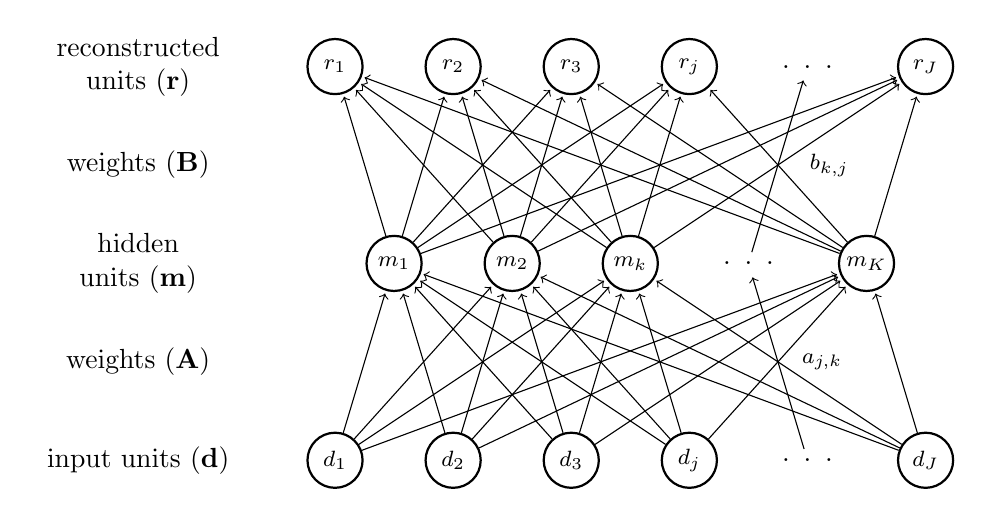
\begin{tikzpicture}[shorten >=1pt,->,draw=black!100]
	\def \rowtwoht{5cm}
	\def \weightstwo{3.75cm}
	\def \rowoneht{2.5cm}
	\def \weightsone{1.25cm}
	\def \basement{0cm}
	\tikzstyle{m-node}=[circle,draw=black!100,thick,inner sep=0pt,minimum size=7mm]
	\tikzstyle{r-node}=[circle,draw=black!100,thick,inner sep=0pt,minimum size=7mm]
	\tikzstyle{d-node}=[circle,draw=black!100,thick,inner sep=0pt,minimum size=7mm]
	\tikzstyle{dots}=[text width=5ex, text centered]
	\tikzstyle{annot}=[text width=17ex, text centered]
	% labels
	\node[annot] (r-layer) at (0cm,\rowtwoht) {reconstructed units ($\mathbf{r}$)};
	\node[annot] (weights) at (0cm,\weightstwo) {weights ($\mathbf{B}$)};
	\node[annot] (hidden-layer) at (0cm,\rowoneht) {hidden units ($\mathbf{m}$)};
	\node[annot] (weights) at (0cm,\weightsone) {weights ($\mathbf{A}$)};
	\node[annot] (d-layer) at (0cm,\basement) {input units ($\mathbf{d}$)};
	
	\node[dots] 	(m3)	at (7.75cm,\rowoneht)	 	{. . .};
	\node[dots] 	(r4) 	at (8.5cm,\rowtwoht)   		{. . .};
	\node[dots] 	(d4) 	at (8.5cm,\basement)   		{. . .};
	
	\footnotesize
	% hidden layer
	\node[m-node] 	(m0)	at (3.25cm,\rowoneht)		{$m_1$};
	\node[m-node] 	(m1)	at (4.75cm,\rowoneht)		{$m_2$};
	\node[m-node] 	(m2)	at (6.25cm,\rowoneht)	 	{$m_k$};
	\node[m-node] 	(m4)	at (9.25cm,\rowoneht)	 	{$m_K$};
	
	% reconstructed vector
	\node[r-node] 	(r0)	at (2.5cm,\rowtwoht)		{$r_1$};
	\node[r-node] 	(r1)	at (4cm,\rowtwoht)		{$r_2$};
	\node[r-node] 	(r2)	at (5.5cm,\rowtwoht)	 	{$r_3$};
	\node[r-node] 	(r3)	at (7cm,\rowtwoht) 		{$r_j$};
	\node[r-node] 	(r5) 	at (10cm,\rowtwoht)   		{$r_J$};
	%\node[r-node] 	(r6) 	at (9.75cm,\rowoneht)   	{$r_J$};
	
	% data vector
	\node[d-node] 	(d0)	at (2.5cm,\basement)		{$d_1$};
	\node[d-node] 	(d1)	at (4cm,\basement)		{$d_2$};
	\node[d-node] 	(d2)	at (5.5cm,\basement)	 	{$d_3$};
	\node[d-node] 	(d3)	at (7cm,\basement) 		{$d_j$};
	\node[d-node] 	(d5) 	at (10cm,\basement)   		{$d_J$};
	%\node[d-node] 	(d6) 	at (9.75cm,\basement)   	{$d_J$};
	
	\path
		(d0)	edge	node	{}	(m0)
		(d0)	edge	node	{}	(m1)
		(d0)	edge	node	{}	(m2)
		%(d0)	edge	node	{}	(m3)
		(d0)	edge	node	{}	(m4)
		%	
		(d1)	edge	node	{}	(m0)
		(d1)	edge	node	{}	(m1)
		(d1)	edge	node	{}	(m2)
		%(d1)	edge	node	{}	(m3)
		(d1)	edge	node	{}	(m4)
		%
		(d2)	edge	node	{}	(m0)
		(d2)	edge	node	{}	(m1)
		(d2)	edge	node	{}	(m2)
		(d2)	edge	node	{}	(m4)
		%
		(d3)	edge	node	{}	(m0)
		(d3)	edge	node	{}	(m1)
		(d3)	edge	node	{}	(m2)
		(d3)	edge	node	{}	(m4)
		%
		(d4)	edge	node[right=2mm]	{$a_{j,k}$}	(m3)
		%
		(d5)	edge	node	{}	(m0)
		(d5)	edge	node	{}	(m1)
		(d5)	edge	node	{}	(m2)
		(d5)	edge	node	{}	(m4)
	 
		(m0)	edge	node	{}	(r0)
		(m0)	edge	node	{}	(r1)
		(m0)	edge	node	{}	(r2)
		(m0)	edge	node	{}	(r3)
		(m0)	edge	node	{}	(r5)

		(m1)	edge	node	{}	(r0)
		(m1)	edge	node	{}	(r1)
		(m1)	edge	node	{}	(r2)
		(m1)	edge	node	{}	(r3)
		(m1)	edge	node	{}	(r5)

		(m2)	edge	node	{}	(r0)
		(m2)	edge	node	{}	(r1)
		(m2)	edge	node	{}	(r2)
		(m2)	edge	node	{}	(r3)
		(m2)	edge	node	{}	(r5)

		(m3)	edge	node[right=3mm]	{$b_{k,j}$}	(r4)	
		
		(m4)	edge	node	{}	(r0)
		(m4)	edge	node	{}	(r1)
		(m4)	edge	node	{}	(r2)
		(m4)	edge	node	{}	(r3)
		(m4)	edge	node	{}	(r5);
		
\end{tikzpicture}
\end{center}
\caption{The ``classical'' autoencoder, one member of the general autoencoder family}
%: an input layer ($\mathbf{d}$), a hidden layer ($\mathbf{m}$), and an output layer
\label{fig:autoencoder}
\end{figure}

%Whereas the MCMM has two layers of nodes ($\textbf{m}$ and $\textbf{r}$), 
 The ``classical'' autoencoder,
shown in figure~\ref{fig:autoencoder} has three layers (or vectors) of nodes:
%, as 
%illustrated in
%in figure~\ref{fig:autoencoder}. 
\begin{enumerate}
\item The \textbf{input} vector $\textbf{d}$
\item The \textbf{hidden} vector $\textbf{m}$
\item The \textbf{output} vector \textbf{reconstruction} layer $\textbf{r}$ 
\end{enumerate}

 Each of these vectors has a counterpart in an MCMM: \textbf{input} vector $\textbf{d}$, $\textbf{m}$, and $\textbf{r}$ vectors are analogous to the vectors of the same name in the MCMM diagram in figure \ref{fig:mcmm}.
However, there are important differences between these two types of autoencoders. The main differences pertain to form (or general architecture), node activation, i.e., the means of computing node activities, and the \emph{optimization procedure}, i.e., method for  minimizing the model's error.

\paragraph{Form.}
Speaking strictly in terms of form, MCMMs and RBMs are identical.
Both are bipartite graphs: Both have two layers of nodes such that there are no direct connections between nodes of the same layer 
%\emph{within} a given layer, all nodes are independent, i.e., a node in one layer can only be connected to nodes of the other later  (That is, there are no connections between nodes of the same the layer. Two nodes can only be be connected if they belong to different layers. of the other layer.)  (connected.)
(see the description of bipartite graphs in chapter~\ref{ch:graph}).  Moreover, in a RBM, as in an \ac{MCMM}, 
one of these node layers functions as a hidden layer, and the other as the visible 
(or surface) layer \citep{mohamed-and-hinton:2010}. 
%\citep[see, e.g.,][]{mohamed-and-hinton:2010}. 
Like MCMMs, RBMs lack an input layer that is distinct from the reconstruction layer. In both MCMMs and RBMs,
the original data vectors $\textbf{x}_i$ are not actually part of the graph, since they are never connected to either the hidden or reconstruction layer (i.e, the the vectors  $\textbf{m}_i$ and  $\textbf{r}_i$, respectively).
In this respect, MCMMs and RBMs differ significantly from the classical autoencoder, wherein the
%In an MCMM, 
%%the oriThe most conspicuous difference is that MCMMs bipartite graph, having just two layers of nodes, namely \textbf{m}$ and \textbf{r}$. Recall that in an MCMM, 
%the original data vector $\textbf{x}$ is actually not part of the graph itself, since it is not connected by weights to either  $\textbf{m}$ or  $\textbf{r}$.
 %In a classical autoencoder, by contrast
%namely the original data vector $\textbf{d}$, the hidden-node vector $\textbf{m}$, and reconstruction vector $\textbf{r}$. These vectors are also present in the MCMM in \ref{fig:mcmm}. One key difference between an MCMM and a classical autoencoder, however, is that the the original data vector 
%$\textbf{d}$ is not a true layer in MCMM, since there are no connecting 
%weights weights between it and $\textbf{m}$ or $\textbf{r}$. This is not 
%the case in a classical encoder, where 
original data vectors $\textbf{x}_i$ constitute a fully integrated layer of the network, namely its input layer, which is distinct from the reconstruction (or output) layer.
\textit{input layer}. Each original data vector $\textbf{x}_i$ enters the network at the input later, is compressed 
at $\textbf{m}_i$, and reconstructed at $\textbf{r}_i$. Because there are three layers 
of nodes in an autoencoder, there must be two layers of weights, labeled 
$\textbf{A}$ and $\textbf{B}$ 
in \ref{fig:autoencoder}. The reconstruction error is computed at $\textbf{r}$, and the appropriate updates are 
\emph{backpropagated} to the $\textbf{B}$ and then $\textbf{A}$ weights.

%Both the \ac{MCMM} and the \ac{RBM} are bipartite graphs.
%Both have two layers of nodes, with no connections between nodes of the 
%same layer (as described in chapter~\ref{ch:graph}).  In a RBM, as in an \ac{MCMM}, 
%one of these node layers functions as a hidden layer, and the other as the visible 
%(or surface) layer \citep[see, e.g.,][]{mohamed-and-hinton:2010}. 
%Consider \eqref{eq:rbm-prob-v} and \eqref{eq:rbm-prob-h}.


%Because an MCMM has no distinct input layer, it is not a directed graph in the same way a 
%that classical autoencoder is a directed graph\footnote{There is a sort of conceptional directionality in an MCMM in that hidden nodes are regarded as ``causing'' the surface units' activities. } 
An MCMM has no designated input layer. The classical autoencoder, by contrast, has distinct input and output layers. Classical autoencoders thus function as a supervised feed-forward neural network. In fact, the only difference between a classical autoencoder and a supervised feed-forward network is that a classical autoencoder's target vectors are its input vectors.

\paragraph{Node Activation.} The RBM and classical autoencoder essentially use the same function for computing node activity values, namely the \emph{sigmoidal weighted sum}.
%are essentially the same, generally  sharing the same activation function.
 However, MCMMs, as we will see, call for a special type of activation function that has different properties to the those of  sigmoidal weighted sum.
 %from one used in RBMs and classical autoencoders. 
%MCMM is significantly different from both the RBM and the classical autoencoder, w

%both in the hidden layer $\textbf{m}$ and the reconstruction layer $\textbf{r}$ is 

The sigmoidal weighted sum is the composition of two functions: the linear weighted sum and the nonlinear logistic sigmoid. 

The weighted sum is the inner product of two vectors, namely the preceding layer's node activities and the corresponding weight vector (i.e., the set of weights linking the preceding node layer to the current layer),
%weight vector connecting preceding layer to the current node in the 
%current layer, 
as in \eqref{eq:sum-m} and \eqref{eq:sum-r}.
The logistic sigmoid \eqref{eq:sig} maps any real number (no matter how large or small) to a number within $[0,1]$.
%composition of the sigmoid function $S$ and the function $t_{i,j}$, 
%which computes a weighted sum, i.e., the inner product of the cluster-activity 
%vector $\mathbf{m}_i$ and the weight vector $\mathbf{c}_j$:


	\begin{equation} %\label{eq:sigws}
	\label{eq:sig}
	\sigma(x) = \frac{1}{1 + e^{-x}} 
	%\quad %\\   %\qquad \text{where} \quad
	%\label{eq:ws}
	\end{equation} %\label{eq:sigws
	
%$p_i =\sigma(a_{i})$
%where $\sigma(x)=frac{1}{1+\text{exp}(-x)}$ is the logistic function. 


%	\begin{equation} %\label{eq:sigws}
%	\label{eq:sig}
%	r_{i,j} =\sigma(t_{i,j}) = \frac{1}{1 + e^{-t_{i,j}}} 
%	%\quad %\\   %\qquad \text{where} \quad
%	%\label{eq:ws}
%	\end{equation} %\label{eq:sigws}
	
%	\begin{align} %\label{eq:sigws}
%	\label{eq:sig-m}
%	m_{i,k} =\sigma(t_{i,k}) &= \frac{1}{1 + e^{-t_{i,k}}} \\
%	\label{eq:sum-r}
%	\text{where} \quad t_{i,k} &= \sum_{j} x_{i,j} a_{k,j}  
%	\end{align}
%	
%	\begin{align} %\label{eq:sigws}
%	\label{eq:sig-r}
%	r_{i,j} =\sigma(t_{i,j}) &= \frac{1}{1 + e^{-t_{i,j}}} \\ %\\   %\qquad \text{where} \quad
%	%\label{eq:ws}
%	\label{eq:sum-r}
%	\text{where} \quad t_{i,j} &= \sum_{k} m_{i,k} b_{k,j} 
%	\end{align}
	
%As noted above, the classical autoencoder, due its tri-layer architecture, requires two sets of weights, $\textbf{U}$ and $\textbf{V}$. 
In a classical autoencoder, the activities of the hidden units are computed via equation \ref{eq:sig-m-ac}. For example, to get the activity of the hidden node $m_{i,4}$ (i.e., $k = 4$), 
we compute the sum $\sum_{j} x_{i,j} a_{4,j}$, where each $x_{i,j}$ is an input node's activity, and $a_{4,j}$ is its corresponding weight in the matrix $\textbf{U}$,
%, which is the equivalent to the inner product \textbf{x}_i \cdot \textbf{c}^{T}_4$ 
and feed the result to the sigmoid function, thus obtaining a final value within $[0,1]$ for each hidden node.
% The weighted sum for each hidden unit activity is  is dot product The weights in $\textbf{U}$ are applied to the network's input layer to compute the activities of the hidden layer. Then the weights  $\textbf{V}$ are applied the newly computed hidden-unit activities to compute the activities of the reconstruction layer. those in $\textbf{V}$ are apply to the hidden layer. 
% On the other hand, RBMs, like MCMMs, have just one, namely $\textbf{C}$. 
	\begin{align} %\label{eq:sigws}
%	\label{eq:sig-m}
	\label{eq:sig-m-ac}
	m_{i,k} &=\sigma(\sum_{j} x_{i,j} u_{k,j}) \\
	\label{eq:sig-r-ac}
  	r_{i,j} &= \sigma(\sum_{j} m_{i,j} v_{k,j}) \\ 
	%&= \frac{1}{1 + e^{-t_{i,j}}} \\ %\\   %\qquad \text{where} \quad
	\end{align}
%	
%	\begin{align} %\label{eq:sigws}
%	\label{eq:sig-r}
%	r_{i,j} =\sigma(t_{i,j}) &= \frac{1}{1 + e^{-t_{i,j}}} \\ %\\   %\qquad \text{where} \quad
%	%\label{eq:ws}
%	\label{eq:sum-r}
%	\text{where} \quad t_{i,j} &= \sum_{k} m_{i,k} b_{k,j} 
%	\end{align}
%For example, to get the activity of the hidden node $m_{i,4}$ (i.e., $k = 4$), 
%we compute the sum $\sum_{j} x_{i,j} a_{4,j}$, where each $x_{i,j}$ is an input node's activity, and $a_{4,j}$ is its corresponding weight in the matrix $\textbf{A}$,
%%, which is the equivalent to the inner product \textbf{x}_i \cdot \textbf{c}^{T}_4$ 
%and feed the result to the sigmoid function, thus obtaining a final value within $[0,1]$ for each hidden node. 
The process is the same for the reconstruction nodes, except that the just-computed hidden-node activities now become the input activities, and the weight vector comes from the $\textbf{V}$ matrix.
% the incoming node activities are those in the hidden layer, and the weight vector is
%the corresponding column in the $\textbf{B}$ matrix.
% Thus, for node, say, 
%$r_{i,6}$ (i.e., $j=6$), the weighted sum is
%%we would sum over the $K$ hidden-unit activities (each multiplied by its respective weight in 
%%$\textbf{b}^{T}_{6}$: 
%$\sum_{k} m_{i,k} b_{k,6}$.  
%%That is, we sum over the $K$ hidden-unit activities, with each activity multiplied by its respective weight in the column (or row?) $\textbf{B}_{:,6}$). 
%We  feed each such sum to the logistic sigmoid function, %as we do for every node. 
%which restrains node activities to the interval $[0,1]$.
%$\textbf{b}^{T}_{6}
% we in the reconstruction vector, specifically The latter takes the output of the linear sum, which could be any real number, possibly much less than 0 or much greater than 1, and maps it onto a number in $[0,1]$.

\begin{figure}[t]
\begin{center}
%\small
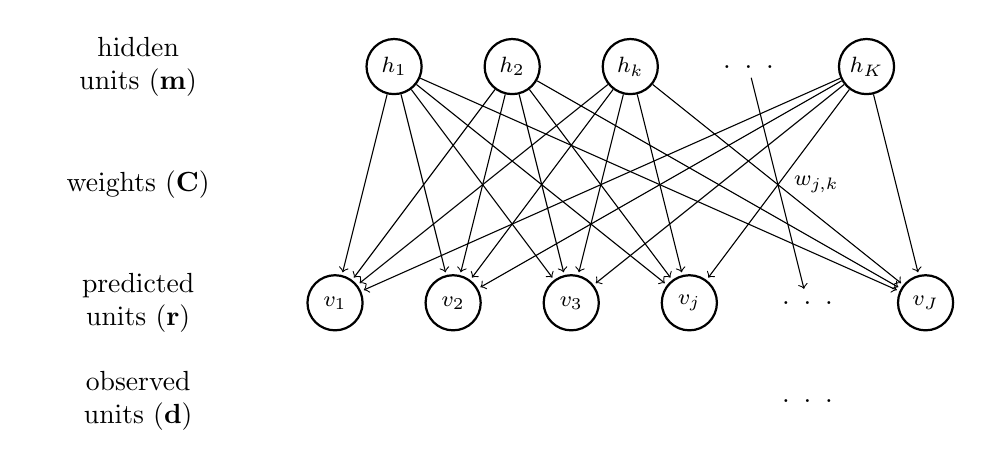
\begin{tikzpicture}[shorten >=1pt,->,draw=black!100]
	\def \rowtwoht{4.25cm}
	\def \weightlevel{2.75cm}
	\def \rowoneht{1.25cm}
	\def \basement{0cm}
	\tikzstyle{m-node}=[circle,draw=black!100,thick,inner sep=0pt,minimum size=7mm]
	\tikzstyle{r-node}=[circle,draw=black!100,thick,inner sep=0pt,minimum size=7mm]
	\tikzstyle{d-node}=[circle,draw=black!100,fill=gray!45,thick,inner sep=0pt,minimum size=7mm]
	\tikzstyle{dots}=[text width=5ex, text centered]
	\tikzstyle{annot}=[text width=17ex, text centered]
	% labels
	\node[annot] (hidden-layer) at (0cm,\rowtwoht) {hidden units ($\mathbf{m}$)};
	\node[annot] (weights) at (0cm,\weightlevel) {weights ($\mathbf{C}$)};
	\node[annot] (r-layer) at (0cm,\rowoneht) {predicted units ($\mathbf{r}$)};
	\node[annot] (d-layer) at (0cm,\basement) {observed units ($\mathbf{d}$)};
	
	\node[dots] 	(m3)	at (7.75cm,\rowtwoht)	 	{. . .};
	\node[dots] 	(r4) 	at (8.5cm,\rowoneht)   		{. . .};
	\node[dots] 	(d4) 	at (8.5cm,\basement)   		{. . .};
	
	\footnotesize
	% hidden layer
	\node[m-node] 	(m0)	at (3.25cm,\rowtwoht)		{$h_1$};
	\node[m-node] 	(m1)	at (4.75cm,\rowtwoht)		{$h_2$};
	\node[m-node] 	(m2)	at (6.25cm,\rowtwoht)	 	{$h_k$};
	\node[m-node] 	(m4)	at (9.25cm,\rowtwoht)	 	{$h_K$};
	
	% reconstructed vector
	\node[r-node] 	(r0)	at (2.5cm,\rowoneht)		{$v_1$};
	\node[r-node] 	(r1)	at (4cm,\rowoneht)		{$v_2$};
	\node[r-node] 	(r2)	at (5.5cm,\rowoneht)	 	{$v_3$};
	\node[r-node] 	(r3)	at (7cm,\rowoneht) 		{$v_j$};
	\node[r-node] 	(r5) 	at (10cm,\rowoneht)   		{$v_J$};
	%\node[r-node] 	(r6) 	at (9.75cm,\rowoneht)   	{$r_J$};
	
%	% data vector
%	\node[d-node] 	(d0)	at (2.5cm,\basement)		{$d_1$};
%	\node[d-node] 	(d1)	at (4cm,\basement)		{$d_2$};
%	\node[d-node] 	(d2)	at (5.5cm,\basement)	 	{$d_3$};
%	\node[d-node] 	(d3)	at (7cm,\basement) 		{$d_j$};
%	\node[d-node] 	(d5) 	at (10cm,\basement)   		{$d_J$};
	%\node[d-node] 	(d6) 	at (9.75cm,\basement)   	{$d_J$};
	
	\path 
		(m0)	edge	node	{}	(r0)
		(m0)	edge	node	{}	(r1)
		(m0)	edge	node	{}	(r2)
		(m0)	edge	node	{}	(r3)
		(m0)	edge	node	{}	(r5)
		
		(m1)	edge	node	{}	(r0)
		(m1)	edge	node	{}	(r1)
		(m1)	edge	node	{}	(r2)
		(m1)	edge	node	{}	(r3)
		(m1)	edge	node	{}	(r5)
		
		(m2)	edge	node	{}	(r0)
		(m2)	edge	node	{}	(r1)
		(m2)	edge	node	{}	(r2)
		(m2)	edge	node	{}	(r3)
		(m2)	edge	node	{}	(r5)
		(m3)	edge	node[right=1mm]	{$w_{j,k}$}	(r4)
		%	
		(m4)	edge	node	{}	(r0)
		(m4)	edge	node	{}	(r1)
		(m4)	edge	node	{}	(r2)
		(m4)	edge	node	{}	(r3)
		(m4)	edge	node	{}	(r5);
		
\end{tikzpicture}
\end{center}
\caption{Restricted Boltzmann Machine} 
\label{fig:rbm}
\end{figure}

An RBM works somewhat differently due to its bipartite architecture. In particular, the \emph{same} matrix of weights---which we are calling $\textbf{C}$ to relate it to the MCMM's architecture---is used both to compute the hidden activities $\textbf{m}$ and the
reconstruction activities $\textbf{r}$. The process is thus bi-directional: The hidden-unit activities are computed via \eqref{eq:sig-m}, and then the reconstruction activities are computed via \eqref{eq:sig-r}. At this point, the reconstruction error is computed, and the weights are updated in proportion to the negative gradient of the error function (REF). Then another round begins: The hidden-unit activities are re-computed from the new reconstruction activities and the updated weights $\textbf{C}$, and then  the reconstruction activities are re-computed from the new hidden-unit activities and the same updated weights $\textbf{C}$. Note that \label{eq:sig-r} and  \label{eq:sig-m} introduce \emph{biases} to weighted sum. These biases are a distinctive feature of RBMs. Like the weights, they are parameters that must be learned
\begin{align}
%\label{rbm:act-v}
\label{eq:sig-r}
%r_{i,j} = P(r_{i,j}|m_{i,k})  = \sigma\big(\sum_{i,k} c_{j,k} m_{i,k}\big)
r_{i,j} &= \sigma\big(\sum_{i,k} c_{j,k} m_{i,k} + a_{k}\big) \\
%\label{rbm:act-h}
\label{eq:sig-m}
m_{i,k} &= \sigma\big(\sum_{j} c_{j,k} r_{i,j} + b_{j}\big) \\
%m_{i,k} = P(m_{i,j}|r_{i,j}) =\sigma\big(\sum_{j} c_{j,k} r_{i,j}\big)
\text{where $a_{k}$ and $b_{j}$ are biases}
\end{align}
But despite these differences, RBM and the classical autoencoder nonetheless share the same basic activation, the sigmoidal weighted sum, a point of significant departure from the MCMM.


The sigmoidal weighted sum is a very common activation function in neural networks, 
but it is not the only way to compute the activity of a node. Any activation function, to borrow
an analogy from \citet{saund:94}, is essentially a voting rule, i.e.,  a policy for combining multiple input votes into a single output decision.  In the context of neural-network models such as RBMs, MCMMs, and classical autoencoders, the output decision is always activity of a given node, and the input votes are the \emph{weighted} activities of the preceding layer's nodes. That is, each vote is a product of the form $h_{k} w_{k,j}$, where $h_{k}$ is the activity of the $k$th hidden node, and $w_{k,j}$ is the weight connecting $h_{k}$ to the node $r_{j}$, whose activity is the question being voted upon. There are always a total of $K$ votes for the activation to take into account, where $K$ is the number of nodes in the preceding layer. 
%wi.e., the products $h_{k} w_{k,j}$ for $k \in K$.
% The question to be
%decided is the activity of $r_{j}$.
%
%is the eand the question to be decided is the activity of a particular node $r_{i,j}$  in the current layer.
%Each vote thus takes the form $h_{k} w_{k,j} $, where $h_{k}$ is a node activity, and $w_{k,j}$ is its weight. 
% should be on or off.  s are the weighted activities of the parent nodes (i.e., the nodes in the preceding layer to which it is connected), a wone layer to yield an activity of a particular node in next/other layer. In graphical models, node activities are generally weighted, and thus each vote in effect takes the form $h_{k} w_{k,j} $, where $h_{k}$ is a node activity, and $w_{k,j}$ is its weight. 

One of the simplest possible activation functions is the sum $\sum_{k} h_{k} w_{k,j}$. It is a possible activation function in that it maps the votes $h_{k} w_{k,j}$ for $k \in K$ to a single output value. However, this value be any real number, one that grows (or shrinks) in direct proportion to the quantity and sizes of its input values. Since most applications require that node activities stay within a certain interval, usually $[0,1]$ or $-1,1]$, the weighted sum's output must be fed to a nonlinear ``squashing'' function, such as the logistic sigmoid, which enforces this constraint.

The sigmoidal weighted sum is in effect a sort of average. To take an average over a set of values is to put them them all in melting pot, so to speak. An average thus tends to obscure the influence of minority subsets of inputs.
%For example, a given month's average temperature cannot be attributed to a few days in that month.  particular inputs as well as minority subsets of inputs.  All input values contribute to the final result, and no individual value is dominant (or such is the assumption in taking an average).
Moreover, the weights in the classical autoencoder range from $-1$ to $1$. 
A negative weight can thus be paired with a positive hidden-unit activity to produce 
a negative vote. The presence of both positive and negative votes means that votes 
can counteract each other and even cancel each other out. 

These properties of the sigmoidal weighted sum allow innumerable possible configurations to produce the same node activity.  \citet{saund:94} argues that this extreme flexibility can be inappropriate when one wants to isolate the particular votes that are responsible for a given surface unit's activity. 
%Thus, sigmoidal weighted sum is, due to its averaging effect, already an unstructured means of combining votes---unstructured in the sense that 
%For instance, suppose one wanted to know the average temperature for the month of July in a certain place. 
%The weighted sum is an extremely flexible method of combining votes. In the classical autoencoder (as well as most neural networks), weights range from $-1$ to $1$. A negative weight can be paired with a positive hidden-unit activity to produce what is in effect a ``negative" vote, allowing votes to cancel each other. The weighted sum is already can thus be configured so that votes cancel one another out. votes can be used to They can thus be configured so that votes can cancel one another,   Moreover, \citet{saund:94} points out that this c
%
%However, because it is linear, its output is proportional to the quantity and sizes of its inputs and thus can be its ou However,  \emph{linear} means of combining the votes of $K$ causal units. \citet{saund:94} argues this summation within the typical sigmoidal update rule can cause a system to learn incoherent weights. for instance that h = [1,0,1] and let $w^1 = [1000,0,-990]$ and $w^2  = [0,0,10]$. Because summation allows arbitrarily large values of opposite signs to counteract each other,
%these to vastly different weight vectors lead the same weighted sum:
%
%\begin{align}
%\sum_{k} h_{k} w^{1}_{k} &= 1000 \times 1  + 0 \times 0 + 1 \times -990 = 10 \\ 
%\sum_{k} h_{k} w^{2}_{k} &= 1 \times 0 + 0 \times 0 +  1 \times 10 = 10
%\end{align}
%
%\cite{saund:94} points out that this behavior obscures the contributions of individual votes. Moreover, the sigmoid function does nothing to remedy this problem; it merely maps large numbers to 1.0 and small numbers to 0 (or values close to 1 and 0, respectively.)

% help the situation. If anything, it further obscures the roles of individual votes. Suppose, for instance, $w^1 = [1000,0,-500]$ 
%and $w^2 = [0,0,100]$, and $h = [1,0,1]$. Then
%\begin{align*}
%\sigma(\sum_{k} h_{k} w^{1}_k}) &= \sigma(500) =  1.0 \\ 
%\sigma(\sum_{k} h_{k} w^{2}_k}) &= \sigma(10) = 1.0
%\end{align*}
As an alternative to the sigmoidal weighted sum and related activation functions, \cite{saund:94} proposes the \emph{mixing function}. Mixing functions are a special class of activation function characterized by their tendency to encourage distinct causal relationships to emerge between hidden and surface nodes.   %that he calls \emph{mixing functions}. 
We shall discuss the properties of mixing functions in greater detail in section~\ref{sec:mixing-function}.


%\cite{saund:94} likens the contribution of each hidden node
%to 
%
%One disadvantage of the sigmoidal weighted sum is
%that it obscures the responsibilities 
%The weighted sum is 
%The MCMM, b	
%This is the mixing (or activation) function that is typically used in classical autoencoders. 
%Whereas the output of Noisy-OR is independent of the number of active 
%causes (as long as there is at least one), the output of \eqref{eq:sig} does
%change with the number of active causes: The value $t_{i,j} = \sum_k m_{i,k} c_{j,k}$ 
%is clearly going to increase as the number of active clusters increases.
%
%%(i.e., products of the form $m_{i,k} c_{j,k}$ that equal $1$ or are greater than some threshold) 
%As $t$ increases, $S(t)$ will get closer to $1$; as %it
%$t_{i,j}$ decreases, $S(t)$ will get closer to $0$.

\paragraph{Optimization procedure.}  In a classical autoencoder, the two layers of 
weights---first $\textbf{B}$ and then $\textbf{A}$---are directly updated via back-propagation. 
But the values of the hidden units are not directly updated; that is, the hidden-unit values 
\emph{depend} on the weights $\textbf{A}$ (along with values in the input vector). 
Thus, in a classical autoencoder, the values of the hidden units change only as a 
consequence of the updates applied to the weights. The same is true in an RBM: an RBM's hidden-unit activities are determined by
the reconstruction units, the weights, and the biases; they are not updated directly.

In an MCMM, by contrast, both $\textbf{m}_i$ and $\textbf{C}$ are \emph{directly} updated. That is, an MCMM requires two complimentary process, \textsc{Optimize-M} and \textsc{Optimize-C} (see \ref{}), each directly manipulating the values in its respective matrix. By contrast,


%MCMM's hidden units are adjusted directly.

 %two layers of weights are updated via back-propagation. 


%Most of the differences between a classical autoencoder and an MCMM stem from the fact that an MCMM is a bipartite graph, whereas a classical autoencoder is not. For instance, because an MCMM has three layers of nodes instead of two,
%it must have two layers of weights.
%Whereas 
%Recall the MCMM, being a bipartite graph, has two 
%layers of nodes, namely the hidden layer \textbf{m}$ and the reconstruction layer 
%$\textbf{r}$ (see figure~\ref{fig:mcmm}. The original data vector 
%$\textbf{d}$ is not a true layer in an MCMM because there are no connections (weights) between it and either \textbf{m}$ 
%or $\textbf{r}$. By contrast, the classical autoencoder has three layers of nodes, as is illustrated in 
%figure~\ref{fig:autoencoder}; these include not only $\textbf{m}$ and $\textbf{r}$, which are analogues to the MCMM's $\textbf{m}$ and $\textbf{r}$ layers), but the original data vector $\textbf{d}$, which is the input layer in a classical autoencoder. Input data vectors are fed to the network via 

% is a true layer in an autoencoder; in particular, it is the input layer.
%: differs from the MCMM in 
%a number of respects. 
%A cursory comparison of the MCMM in figure~\ref{fig:mcmm} and the classical auto-encoder in 
%figure~\ref{fig:autoencoder} reveals clear structural differences, the most immediately apparent 
%of which is that whereas MCMM has one layer of connecting weights, labeled $\textbf{C}$ in 
%figure~\ref{fig:mcmm}, the classical autoencoder as 
%two. These are labeled $\textbf{A}$ and $\textbf{B}$ in figure~\ref{fig:autoencoder}.
%
%First, notice in figure~\ref{fig:autoencoder}, that a classical autoencoder has two whereas an MCMM has a single layer of connecting weights, labeled $\textbf{C}$ in figure~\ref{fig:mcmm}, a classical autoencoder has two

%Under this general definition of \emph{autoencoder}, the ``classical'' autoencoder is a particular subtype of autoencoder. 
%should reduce the reconstruction error then measures the This   That is, an algorithm that seeks to learn a compressed representation a its input data such that the original input data can be \emph{reconstructed} from the compressed representation.   an internal model of the input data from which  wherein the autoencoder learn a compressed representation of its input data that  and then tests this representation by trying to generate of the data by attempting to generate (or \emph{reconstruct}) the original input data from it and then measuring of the error between the reconstructed and original data points. The autoencoder's internal A single iteration in an autoencoder's learning process consists of the following general steps: 
%\begin{enumerate}
%\item compression
%\end{enumerate}
%(1) compression, (2) reconstruction, (3) error calculation, (4) adjustment measurement step, i.e., of the \emph{reconstruction error}, the discrepancy between the reconstructed data and the original data. 


%f titeratively positing such an encoding and then trying to reconstruct the input data vectors from it. If there is \emph{reconstruction error}, it makes appropriate adjustments to the encoding, computes new reconstructions, and so on, until the discrepancy between the original and reconstructed data vectors is minimized.
%
%In addition to the MCMM, one autoencoder subtype is of course the ``classical'' autoencoder, 
%depicted in figure~\ref{fig:autoencoder}. This is the canonical autoencoder, and we thus consider its structure first in order to set up our discussion of the MCMM's structure. Later in this section, we will discuss yet another
%autoencoder subtype, the Restricted Boltzmann Machine (RBM). By contrasting the MCMM with these two other
%autoencoders, we will cast the MCMM's structure into sharper relief.
%
%
%i.e., a compressed representation of its input data---a model of its latent structure---that generates its input data. That hidden structure of its input data by iteratively positing a model of the (or model, theory, etc.) of its input data from which its original input data from which the input 



% First, there is a generic autoencoder concept
% The generic autoencoder concept has several subtypes.

%Both hidden nodes and surface nodes have activity values, i.e., values in $[0,1]$ that
%indicate whether a node is \textsc{on} (active) or \textsc{off} (inactive). Each surface-node activity 
%is a function of the hidden-node activities and the weights that connect the hidden nodes to the surface node in question.

%Each surface node is either \textsc{on} (active) or \textsc{off} (inactive) depending 
%on the hidden-node activities and
%the weights connecting hidden nodes to surface nodes. 

%\subsection{Architecture}
%\label{subsec:architecture}

%An MCMM can be viewed as a variant of the classical autoencoder
%network \citep{dayan-and-zemel:95}, a type of neural network used for
%unsupervised learning.  In autoencoders, a hidden layer is forced to
%learn a compression scheme, i.e., a lower-dimensional encoding, for
%a dataset.
 
%MCMMs are called \emph{Multiple Cause} Mixture Models because more
%than one hidden unit can take part in the activation of a surface
%unit.  
%This is illustrated in figure \ref{fig:mcmm}, where the nodes
%$\mathbf{m}$ are the hidden units, and $\mathbf{r}$ is the (reconstructed) surface
%vector.
%Each arc $c_{j,k}$ represents the weight on the connection between
%$m_k$ and $r_j$.
%The activity of $r_j$ is determined by a mixing function 
%(section~\ref{sec:mixing-function}).




% in $\textbf{c}_{j}$.

%From source: "One  can  qualitatively  understand  the  difference  between  mixtures  and  products  by  observing  that  admixture distribution can have high probability for events when only a single expert assigns high probability to that event.  In contrast, a product can only have high probability for an events when all experts assign high probability to that event.  Hence, metaphorically speaking, a single expert in a mixture has the power to pass a bill while a single expert in a product has the power to veto it.Put another way, each component in a product represents a soft constraint, while each expert in a mixture represents a soft template or prototype. For an event to be likely under a product model, all constraints must1
%be (approximately) satisfied, while an event is likely under a mixture model if it (approximately) matches with  a  single  template."

%Bishop: "One approach is to apply gradient-based optimization techniques (Fletcher, 1987;Nocedal and Wright, 1999; Bishop and Nabney, 2008). Although gradient-based techniques are feasible, and indeed will play an important role when we discuss mixture density networks in Chapter 5, we now consider an alternative approach known as the EM algorithm which has broad applicability and which will lay the foundations for a discussion of variational inference techniques in Chapter 10." p. 435

%% Quora: "LDA is not a mixture model.  It is an admixture model or a mixed-membership model.
%Mixture models have a single latent variable that denotes which cluster they're in.  This is often written as an indicator variable z.  
%LDA is a model over documents (a bag of words), and has a latent variable for topic assignments for every token:  z1?zN
%Thus, words can belong to different clusters.  This intuitively makes sense because documents can be about more than one thing.  I.e., about both technology and business.  This often results in better models of real text than pure mixture models."

%The MCMM learns by comparing the reconstructed vector $\mathbf{r}_i$ 
%to its corresponding original datapoint $\mathbf{d}_i$. The discrepancy between
%the two is quantified by an \emph{objective function}. 
%If there is a discrepancy, the values of the nodes in
%$\mathbf{m}_i$ as well as the weights $\mathbf{C}$ are adjusted 
%in order to reduce the discrepancy as much as possible.
%See section~\ref{sec:mcmm-learning} for more on the learning process.

%Suppose data points $\mathbf{d}_u$ and $\mathbf{d}_v$ have some features in common.
%Then, as the MCMM tries to reconstruct them in $\mathbf{r}_u$ and $\mathbf{r}_v$, respectively,
%similarities will emerge between their respective hidden-layer vectors $\mathbf{m}_u$ and $\mathbf{m}_v$.
%In particular, the vectors $\mathbf{m}_u$ and
%$\mathbf{m}_v$ should come to share at least one active node, i.e., at least
%one $k \in K$ such that $m_{u,k} = 1$ and $m_{v,k} = 1$.
%This can serve as a basis for clustering;
%i.e., $m_{i,k}$ indicates whether $\mathbf{d}_i$ is a member of cluster $k$.

\subsection{Mixture and Mixed-Membership Models}

A mixture model attempts to account for the data points in a data set by assuming that multiple probability
distributions are responsible for generating the data. It also assumes that each data point is generated
by exactly one of these underlying distributions. These underlying distributions can be interpreted as clusters, in which case each data point is assigned to one of multiple clusters. However, since the process is probabilistic,
data points are generally not mapped to clusters with 100 percent certainty. There may be, for example, a 60 percent chance a datapoint belongs to one cluster, a 30 percent chance it belongs to another, and a 10 percent change it belongs to yet another. In a \emph{hard clustering}, the data point is assigned to the most probable category, and the other less probable possibilities are forgotten. However, sometimes the uncertainty is left unresolved, so that, in the case of our example, all three possibilities, along with their respective likelihoods, would be output. This is a \emph{soft} clustering. But even in the case of a \emph{soft} clustering, we still assume that the data point in question belongs to only one cluster; the ``softness" of the clustering just expresses the model's uncertainty about which cluster this is. %the data point belongs.

By contrast, a mixed-membership model, e.g. Latent Dirichlet Allocation \citep{blei-et-al:2003},
%\footnote{
%Like latent Dirichlet allocation, MCMMs have
%been applied to document classification; \cite{sahami-et-al:96} 
%use an \ac{MCMM} to group $I$ documents into $K$ clusters.  Documents are 
%represented as vectors $\mathbf{x}_i$ of $J$ features. The features, i.e. surface units, 
%each indicate the absence or presence of a particular word (cf. the $\mathbf{x}$ 
%vector in figure~\ref{fig:mcmm}). The topics in \cite{sahami-et-al:96} are represented 
%as the MCMM's hidden units $\mathbf{m}_i$. Documents are grouped into topic 
%clusters by the learning process described below in section~\ref{sec:mcmm-learning}.}, 
views data points as complex objects, i.e., as themselves consisting of multiple objects, 
each of which is generated by one of multiple probability distributions (or clusters). 
For example, in a mixed-membership \textit{topic model}, the complex objects are the 
\emph{documents} within a given corpus. The simple or elemental objects that compose 
the documents are \emph{words}. The clusters correspond to \emph{topics}, which generate 
the words that compose the documents. That is, each document is a set of words, and each 
word is generated by a particular topic. The document is associated to (or ``becomes a member of'') each topic that is
responsible for at least some of its words. 

However, these topics generally cannot all claim equal responsibility
for the document. One topic might be responsible for 40 percent, for instance,
of the words, another for 30 percent, and so on. A single topic can not be responsible for the whole 
document unless no other topics are involved.  However, it is important to note that these 
percentages do not indicate uncertainty as they would in mixture models. The assumption
of multiple causes (i.e., clusters) is built 
into mixed-membership models, whereas mixture models assume a single cause for each 
data object. The reason that mixed-membership models yield percentages is 
that they decompose each data object into many elemental objects and allow different causes (e.g., topics) to claim responsibility for different elemental objects within the same document. 

Like mixed-membership models, multiple-cause mixture models (MCMMs) allow multiple causes to take part in accounting for a single data point. That is, as in mixed-membership models, MCMMs provide a means for different causes to take responsibility for different parts of data point. Thus, both MCMMs and mixed-membership models transcend standard mixture models and their assumption that each data point ultimately has only one cause. % (with or without uncertainty)

MCMMs differ from mixed-membership models in that MCMMs do not deal in 
percentages; that is, in MCMMs, a cause (or cluster) cannot be, for instance, 
40 percent responsible for a (complex) data object. Rather, in MCMMs, 
cluster membership is binary: either True or False---100 percent or 0 percent, as it were. 
This behavior is a consequence of MCMMs' mixing functions (see section~\ref{sec:mixing-function}). 
MCMMs do allow individual clusters to claim responsibility for particular features (i.e., individual components within data points). This is in fact a key property of MCMMs. 
The difference between MCMMs and mixed-membership models stems from 
both the neural nature and the mixing functions MCMMs: An MCMM's mixing 
function requires a hidden unit's activity to be 1 in order for it count as an 
``\textsc{on}'' vote for a particular surface unit, and 0 to be an ``\textsc{off}'' vote. 
Of course, during learning, many hidden-unit activities will be between 0 and 1, 
but the learning process pushes them ever closer to one of these two values. 
Activity values between 0 and 1 can be interpreted as``almost off" and ``almost on," 
but not as real percentages as in mixed-membership models. 

This binary treatment of causes in MCMMs is arguably more suitable for morphological learning than a framework that assigns `` ownership percentages'' to causes.  We generally do not think of words' morphological compositions in terms of percentages.  That is, we tend not to say things like, ``60 percent of this word belongs to this morphological category, and 40 percent belongs to that category." Of course, such a statement would be particularly incoherent if we were speaking in terms of morphosyntactic categories, such as past tense. But it is also problematic in the case of form-based categories. Proportions of characters (or form-describing binary features) simply do not have a meaning in morphology, not one comparable to the that of word proportions in topic modeling, at any rate. In morphology, it is the presence/absence of a morphological unit that is important, not the proportion of characters or features it claims within the word
Moreover, the percentages of mixed-membership models can be interpreted as degrees of membership:  
``[M]ixed membership models assume that individuals or observational units [i.e., words] may only partly belong to population mixture categories [i.e., topics] \dots. The degree of membership then is a vector of continuous, non-negative latent variables [i.e., hidden units] that add up to 1'' \citep[][p. 4]{airoldi-et-al:2014}. In neither actual morphology nor in an MCMM are there degrees of membership, nor a requirement that they should add up to one for any given word. 

\begin{table}{htb}
\centering
\begin{tabular}{ccc}
Topic-Modeling & & ULM \\
document & $\to$ & word \\ %(i.e, feature-vector representing a word) \\
topic & $\to$ & morph/morpheme \\
word & $\to$ & word-internal feature or character \\
\end{tabular}
\caption{Some topic-modeling terms and their ULM equivalents. That is, for instance, \emph{documents}
in the context of topic modeling are equivalent to \emph{words} in the context of the unsupervised learning
of morphology.}
\label{tab:tm-to-ulm}
\end{table}	

				
\section{Mixing Function}
\label{sec:mixing-function}

In this section, we discuss the \emph{mixing function}, 
the component within an MCMM responsible for determining activities of the surface nodes $\textbf{r}_i$.
% based on the activities of the hidden units and weights. That is, 
%To output the activity of the $j$th surface node, i.e., $\textbf{r}_{i,j}$, a mixing function 
A mixing function takes as input the hidden-unit activities accompanied by the weights 
linking the hidden units to a particular surface node, and outputs the activity 
for this surface node. and their corresponding weights is  multiplied by 
particular vector weights---and outputs the activity of a particular surface 
(or reconstruction) node.  \citet{saund:94} describes mixing functions in terms of 
\emph{voting rules}, i.e., rules for combining multiple votes to yield a single decision, 
where the votes are the products $m_{i,k}c_{j,k}$ for $k \in K$, and the decision an 
activity value for the $j$th surface node $\textbf{r}_{i,j}$. All mixing functions
are activation functions, but not all activation functions are mixing functions.
That is, mixing functions constitute a special class of activation function; they are 
activation functions
specially tailored to serve the needs MCMMs. These needs are essentially as follows:
\begin{enumerate}
\item Each of $K$ the hidden-unit activities for a given data point (i.e., word) 
must be interpretable as binary indicators of cluster membership, where $1$ 
indicates membership, and $0$ non-membership. Thus, a given word belongs to the 
$k$th cluster if its $k$th hidden-unit activity is $1$.
\item The $j$th vector of weights $\textbf{c}_j$ (i.e., the $j$th row 
of the weight matrix $\textbf{C}$) must be interpretable as the centroid 
(i.e., the ``average" vector) of the $k$th cluster. 
\end{enumerate}
In short, both the hidden-unit values and weights must have coherent interpretations. 
Recall from section~\ref{sec:context} that the sigmoidal weighted sum is 
an activation function that does not satisfy these criteria. It does not encourage 
a network to learn interpretable valuations for parameters. It therefore is 
not mixing function. All mixing functions
are activation functions, but not all activation functions are mixing functions.
%That is, mixing functions are a special class of activation function

%We have distinguished two different types of multiple cause binary data do
%main and have shown that appropriately tuned mixing functions—quite
%different from the standard linear sum followed by sigmoid squashing—
%permit recovery of the component cluster features.

Just as there are many possible activation functions, there are many possible mixing functions.
\citet{saund:94} proposes two, each specially designed for a particular kind of problem or ``data domain.'' These
domains, which Saund calls the ``\textsc{write-black}'' (WB) and the ``\textsc{write-white-or-black}'' (WWB) domains, are distinguished by the nature of the voting scheme that determines the values of the surface
nodes. In the \textsc{write-black} domain, the decision in question is whether a given surface unit should be ``black" (i.e., 1) or ``not black'' (i.e., 0). The votes for each such decision are 1 or 0 (or between 1 and 0 prior to convergence) and combined according to the  Noisy-Or mixing function \citep{pearl:1988}, defined in \eqref{eq:noisy-or}.
\begin{equation}\label{eq:noisy-or}
r_{i,j} = 1 - \prod\limits_{k} (1 - m_{i,k} c_{j,k})
\end{equation}
% We will call the inputs to the Noisy-OR function \emph{causes}. Each cause is a product of the form $m_{i,k} c_{j,k}$. 
 The Noisy-OR function is essentially an\textit{OR} gate, or, to put it another way, 
 an``at-least-one" gate. That is, the surface node $r_{i,j}$ is $1$ as long as 
 \emph{at least one} cause is active.
 % (i.e., $m_{i,k} c_{j,k} = 1$ for at least one $k$ in $K$). 
 If two or more causes are active,
%$1$ (or $\ge$ than a threshold), 
$r_{i,j}$ is still going to be $1$. The output of Noisy-OR does not change 
as the number of active causes changes; it is 1 as long as there is at least one active cause.

%Saund calls one the \textsc{write-black} (WB) domain, wherein votes are in the interval $[0,1]$ (and eventually either 0 or 1 as the model approaches convergence) and the other the 
The \textsc{write-white-or-black} domain differs from \textsc{write-white-or-black} in that requires that the mixing function be capable of outputting negative surface-unit activities as well as positive. The Noisy-OR function thus will not work as a mixing function in this case. Saund instead proposes the function defined in \eqref{eq:wwb}. gsurface units can be negative as well as positive, i.e., 1 for ``black'' and -1 for ``white."  The votes in this scenario are in the interval $[-1,1]$.

 \begin{align}\label{eq:wwb}
  r_{i,j} &=
    \begin{cases}
      \frac{\sum\limits_{k} m_{i,k} c_{j,k}}{\sum\limits_{k} m_{i,k} |c_{j,k}|} & \text{$\forall m_{i,k}, c_{j,k} : m_{i,k} c_{j,k} \in \{-1,0,1\} $}\\
      0 & \text{if \, $\sum\limits_{k} m_{i,k} |c_{j,k}|= 0$}\\
    \end{cases} \\
    %\end{align}
%& \text{where}
%\begin{cases}
%%\text{observed data: $x_{i,j} \in \{-1,1\}$} \\
%\text{$-1 \leq  c_{j,k} \leq 1$ \quad (weights)} 
%\text{measurements: $0 \leq  m_{i,k} \leq  1$ \quad (hidden units)} 
%& \text{predictions: $-1 \leq  r_{i,j} \leq  1$} 
%\end{cases}
 \end{align}
where $c_{j,k} \leq 1$, $0 \leq  m_{i,k} \leq  1$,  $-1 \leq  r_{i,j} \leq  1$, 
and the components $x_{i,j}$ of the original data points
are each either $1$ or  $-1$. Note the absolute value in the denominator 
of the expression $\frac{\sum_{k} m_{i,k} c_{j,k}}{\sum_{k} m_{i,k} |c_{j,k}|}$. 
This absolute value allows the numerator and denominator to differ in sign so that 
the output $r_{i,j}$ can be either positive or negative and thus match components of the original data points.

 Interestingly, \eqref{eq:wwb} contains the same weighted sum 
 as the sigmoidal weighted sum. There are, however, important differences 
 between \eqref{eq:wwb} and the sigmoidal weighted sum. First, there is 
 no logistic sigmoid in \eqref{eq:wwb}; it is the denominator $\sum_{k} m_{i,k} |c_{j,k}|$ 
 that constrains output of \eqref{eq:wwb} to the interval $[-1,1]$. The other 
 difference is the nonlinearity arises from the conditions on the output \eqref{eq:wwb}; 
 to avoid division by zero, it is necessary to stipulate that $r_{i,j}=0$ if 
 $\sum_{k} m_{i,k} |c_{j,k}| = 0$, a result that occurs only if every vote is 0, 
 in which case no cluster can claim responsibility for the value of $r_{i,j}$. But 
 because $0$ never occurs in the original data points in the \textsc{write-white-or-black} 
 domain, the learning process would tend drive activities of the reconstruction nodes 
 away from $0$. That is, because the learning process seeks to minimize the discrepancy 
 between $\textbf{r}_i$ and $\textbf{x}_i$, $0$ cannot a valid final value for any $r_{i,j}$.  
 Thus, the weights and the hidden-unit vectors will be shaped to produce surface-node 
 activities that are either $-1$ or $1$ in accordance with the component values of 
 the original data points. 

To ensure that the activity of $r_{i,j}$ is either $-1$ or $1$, at least one hidden 
unit $m_{i,k}$ must have an activity of 1, and the weight associated with this 
hidden unit, namely $c_{j,k}$, must be either $-1$ or $1$. This would tie 
the surface unit $r_{i,j}$ to at least one cluster. Ultimately, the mixing 
function \eqref{eq:wwb} encourages hidden-unit activities to move  toward 
either $0$ or $1$ and the weights toward either $-1$ and $1$. These are 
values with clear cluster-oriented interpretations: The $1$'s and $0$'s of the 
hidden-unit activities indicate cluster membership and nonmembership, respectively, 
while the weights adopt the same pair of values present in the original data points. 
This is important, since, as noted above, an MCMM's weight vectors have to be 
interpretable as cluster centers, i.e., the composite or average of that cluster's 
member data points. %take on the same values-1 and 1 as weight values correspond to the component values of the original data points, 
%each vote will ultimately be pushed toward $1$ or $-1$, meaning that each hidden unit activity $m_{i,k}$ will be pushed toward either 0 
%an  $m_{i,k}c_{j,k}$
%is actually a class of All mixing functions
%are activation functions, but not all activation functions are mixing functions.
%That is, mixing functions are a special class of activation function (see section~\ref{sec:context}). 
%, we descri.from hidden units' activities paired with the appropriate weights (i.e., the products
%$m_{i,k}c_{j,k}$ for $k \in K$) and combines them to yield a 
%\emph{weighted} activity values $outputs the values of the reconstruction (surface) nodes $\mathbf{r}$. In particular, 

In preliminary experiments for the present work, I tried both the Noisy-OR 
and the \textsc{Write-White-or-Black} mixing functions. The latter did 
not work well; in fact, under the \textsc{Write-White-or-Black}, the system 
was unable to make progress toward learning to reconstruct the original 
data points. This may have been due to the sparseness of the data points 
in this study; each data point is vector of hundreds of feature slots, but 
only a handful have the value $1$. are feature-vector representations of words. 
There are hundreds of features, and each there is a slot for each feature in each 
feature. If the feature is present in the word in question, its slot 
(We will discuss these features in detail in chapter~\ref{ch:experi}.)

%in fact, it seemed to be fundamentally ill-suited to the present study's learning task. proved not to work well given for the purposes of the present study,  particularly the nature of this study's data points. Recall this study's data points are feature-vector representations of words, and that these feature vectors are sparse. That is, for any given word, most features are not present. 
In a \textsc{Write-Black} formulation, absent features have the value $0$, but in the write-white-or-black formulation, they are $-1$. Therefore, in a sparse feature vector under the write-white-or-black formulation, the vast majority of features are $-1$. The cumulative effect of all these negatives in \eqref{eq:wwb} seemed to drown out the few positive positive features, making it impossible to reproduce the original data vectors. 

Noisy-OR, on the other hand, did allow learning to take place; that is, 
the system was able to reduce its error with Noisy-OR as its mixing function. 
Apparently, this study's sparse feature vectors (i.e., data points) are more aptly 
placed in the \textsc{Write-Black} domain than the \textsc{Write-White-or-Black} domain.
%proved to more amenable the present study's learning task, including to allow learning. amenable to sparse feature vectors as well as other aspects of this study approach to morphological learning. I therefore adopted Noisy-Or as the mixing function for Multimorph's MCMM. 

%that detewhich is a kind of activation function to the  perhaps the most significant component 
%The mapping between the layer of hidden nodes $\mathbf{m}$ 
%and the layer of surface nodes $\mathbf{r}$ is governed by a 
%\emph{mixing function}, which is essentially
%a kind of voting rule \citep{saund:94}. That is, maps from a set of (weighted)
%input ``votes'' to a single output decision.  The output decision is 
%an activity value for a particular surface-layer node. We will call the input votes
%\emph{causes}. 

%Each cause is a product of the form $m_{i,k} c_{j,k}$ for $k \in K$.
%There are thus a total of $K$ distinct causes for a given surface node $r_{i,j}$. 
%If the cause $m_{i,h} c_{j,h}$, where $h \in K$, is equal to $1$ or surpasses some
%threshold, then $m_{i,h} c_{j,h}$ is an active cause.

\begin{figure}[htb]
\begin{center}
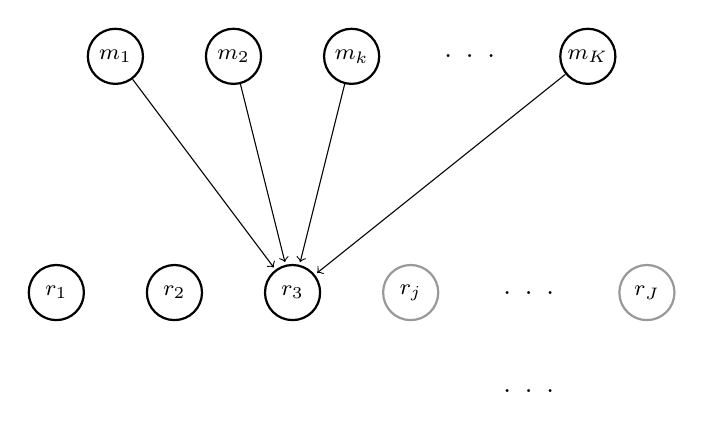
\begin{tikzpicture}[shorten >=1pt,->,draw=black!100]
	\def \rowtwoht{4.25cm}
	\def \weightlevel{2.75cm}
	\def \rowoneht{1.25cm}
	\def \basement{0cm}
	\tikzstyle{m-node}=[circle,draw=black!100,thick,inner sep=0pt,minimum size=7mm]
	\tikzstyle{r-node}=[circle,draw=black!100,thick,inner sep=0pt,minimum size=7mm]
	\tikzstyle{r-node-2}=[circle,draw=black!40,thick,inner sep=0pt,minimum size=7mm]
	%\tikzstyle{d-node}=[circle,draw=black!100,fill=gray!45,thick,inner sep=0pt,minimum size=7mm]
	\tikzstyle{dots}=[text width=5ex, text centered]
	%\tikzstyle{annot}=[text width=17ex, text centered]
%	% labels
%	\node[annot] (hidden-layer) at (0cm,\rowtwoht) {hidden units ($\mathbf{m}$)};
%	\node[annot] (weights) at (0cm,\weightlevel) {weights ($\mathbf{C}$)};
%	\node[annot] (r-layer) at (0cm,\rowoneht) {predicted units ($\mathbf{r}$)};
	%\node[annot] (d-layer) at (0cm,\basement) {observed units ($\mathbf{d}$)};
	
	\node[dots] 	(m3)	at (7.75cm,\rowtwoht)	 	{. . .};
	\node[dots] 	(r4) 	at (8.5cm,\rowoneht)   		{. . .};
	\node[dots] 	(d4) 	at (8.5cm,\basement)   		{. . .};
	
	\footnotesize
	% hidden layer
	\node[m-node] 	(m0)	at (3.25cm,\rowtwoht)		{$m_1$};
	\node[m-node] 	(m1)	at (4.75cm,\rowtwoht)		{$m_2$};
	\node[m-node] 	(m2)	at (6.25cm,\rowtwoht)	 	{$m_k$};
	\node[m-node] 	(m4)	at (9.25cm,\rowtwoht)	 	{$m_K$};
	
	% reconstructed vector
	\node[r-node] 	(r0)	at (2.5cm,\rowoneht)		{$r_1$};
	\node[r-node] 	(r1)	at (4cm,\rowoneht)		{$r_2$};
	\node[r-node] 	(r2)	at (5.5cm,\rowoneht)	 	{$r_3$};
	\node[r-node-2] 	(r3)	at (7cm,\rowoneht) 		{$r_j$};
	\node[r-node-2] 	(r5) 	at (10cm,\rowoneht)   		{$r_J$};
	%\node[r-node] 	(r6) 	at (9.75cm,\rowoneht)   	{$r_J$};
	
	% data vector
%	\node[d-node] 	(d0)	at (2.5cm,\basement)		{$d_1$};
%	\node[d-node] 	(d1)	at (4cm,\basement)		{$d_2$};
%	\node[d-node] 	(d2)	at (5.5cm,\basement)	 	{$d_3$};
%	\node[d-node] 	(d3)	at (7cm,\basement) 		{$d_j$};
%	\node[d-node] 	(d5) 	at (10cm,\basement)   		{$d_J$};
	%\node[d-node] 	(d6) 	at (9.75cm,\basement)   	{$d_J$};
	
	\path 
		(m0)	edge	node	{}	(r2)
	
		(m1)	edge	node	{}	(r2)

		(m2)	edge	node	{}	(r2)
		%(m3)	edge	node {}	(r4)
		%(m3)	edge	node[right=1mm]	{$c_{j,k}$}	{}	(r0)
		%	
		(m4)	edge	node	{}	(r2);

		
\end{tikzpicture}
\end{center}
\caption{%The activity of each surface unit  is determined by a \emph{vote}, so to speak.  
Each hidden unit casts a \emph{weighted vote}, so to speak, to decide the activity of a given surface (or reconstruction) unit.}
%i.e., a value eThe votes must then be combined in some way to yield an activity.}
%$r_{i,j}$
% Each hidden unit $m_{i,k}$ casts a weighted vote, i.e., the product $m_{i,k}c_{j,k}$. 
% The votes must then be combined in some way to yield a single activity for $r_{i,j}$.}
\label{fig:voting}
\end{figure}

% \begin{align}\label{eq:wwb}
%  r_{i,j} &=
%    \begin{cases}
%      \frac{\sum\limits_{k} m_{i,k} c_{j,k}}{\sum\limits_{k} m_{i,k} |c_{j,k}|} & \text{$\forall m_{i,k}, c_{j,k} : m_{i,k} c_{j,k} \in \{-1,0,1\} $}\\
%      0 & \text{if \, $\sum\limits_{k} m_{i,k} |c_{j,k}|= 0$}\\
%    \end{cases} \\
%& \text{where} \\
%%\text{observed data: $x_{i,j} \in \{-1,1\}$} \\
%& \text{$-1 \leq  c_{j,k} \leq 1$ \quad (weights)} \\
%& \text{measurements: $0 \leq  m_{i,k} \leq  1$ \quad (hidden units)} 
%& \text{predictions: $-1 \leq  r_{i,j} \leq  1$} 
%\end{align}
%Note that when any activity $m_{i,k} = 0$, that cluster-center drops out from 
%having any influence on the predictions $r_{i,j}$ and the effective dimensionality of the hypercube decreases by 1.

%In its architecture, MCMMs bear a striking resemblance to the 
%Restricted Boltzmann Machine (RBM) \citep{smolensky:1986}. 
%In particular, both the \ac{MCMM} and the \ac{RBM} are bipartite graphs. That is,
%like an MCMM, an RBM has two layers (or sets) of nodes such that no two nodes within the same layer are connected.  connections only, as described in chapter~\ref{ch:graph}). In addition, the RBM literature typically uses the terms \emph{hidden} and \emph{visible} to refer to these two layers, where \emph{visible} is analogous to (and synonymous with) our term \emph{surface}. Moreover, learning in both MCMMs and RBMs is the result of an effort to reconstruct the actual data vectors in the surface (or visible) layer.

% one of the RBM layers is typical called the \emph{visible} layer,  hiddenas eter has a layer of hidden nodes and a layer of surface (or \emph{visible}) nodes. In the RBM literature, the surface layer is usually called the ``visible'' layer, but the two terms are synonymous. \footnote{In the RBM literature, authors typically the symbols $\textbf{h}$ and $\textbf{v}$ to refer to the hidden and visible (or surface) layers, respectively, whereas we are using $\textbf{m}$ and $\textbf{r}$, respectively, to refer the MCMM's hidden and surface layers.} 
%To make clear the correspondence between RBMs and MCMMs, let us apply the same set symbolfigure~\ref{fig:mcmm} to refer an RBM's components: 
%That is, in both, there are two layers of nodes---a hidden layer and a surface (or visible) layer, and there are no connections between nodes of the 
%same layer, as described in chapter~\ref{ch:graph}).
%Like an MCMM, an RBM is a bipartite graph. 
%There are important differences, however. 
%
%Both the \ac{MCMM} and the \ac{RBM} are bipartite graphs.
%That is, both have two layers of nodes, with no connections between nodes of the 
%same layer (as described in chapter~\ref{ch:graph}).  In a RBM, as in an \ac{MCMM}, 
%one of these node layers functions as a hidden layer, and the other as the visible 
%(or surface) layer \citep[see, e.g.,][]{mohamed-and-hinton:2010}. 
%Consider \eqref{eq:rbm-prob-v} and \eqref{eq:rbm-prob-h}.
%\begin{equation}\label{rbm:act-v}
%r_{i,j} = P(r_{i,j}|m_{i,k})  = \sigma\big(\sum_{i,k} c_{j,k} m_{i,k}\big)
%\end{equation}
%\begin{equation}\label{rbm:act-h}
%m_{i,k} = P(m_{i,j}|r_{i,j}) =\sigma\big(\sum_{j} c_{j,k} r_{i,j}\big)
%\end{equation}
%$p_i =\sigma(a_{i})$
%where $\sigma(x)=frac{1}{1+\text{exp}(-x)}$ is the logistic function. 
%\begin{align}
%P(v|h) &= \prod_{i=1}^m P(v_i|h)  \label{eq:rbm-prob-v}\\
%P(h|v) &= \prod_{j=1}^n P(h_j|v) \label{eq:rbm-prob-h}
%\end{align}



%\begin{equation} \label{eq:rbm-prob-v}
%P(v|h) = \prod_{i=1}^m P(v_i|h)
%\end{equation}
%\begin{equation}  \label{eq:rbm-prob-h}
%P(h|v) &= \prod_{j=1}^n P(h_j|v)
%\end{equation}
 

%********
%One difference between 
%the two, however, is that an RBM acts as a \emph{product} of experts, while an \ac{MCMM} 
%acts as a kind of hybrid between a \emph{mixture of experts}, i.e., a (standard) mixture model, 
%and a product of experts. To be clear, though, an \ac{MCMM} itself appears to be neither
% a sum nor a product of experts, not at least as these terms are usually construed. 
%
%
%The ``experts" here 
%%The RBM's equivalent of an MCMM's mixing function is a  \emph{product of experts}\citep{hinton:1999, hinton:2002}, where the ``experts" 
%are the hidden units (along with their
%respective weights). A product of experts is, as its name suggests, a multiplication, 
%namely the product of all hidden-unit values, whereas a mixture of experts is a 
%summation of these same values. In both MCMMs and RBMs, every expert casts 
%a vote concerning whether a given surface node is to be \textsc{on} or \textsc{off} 
%(i.e., 1 or 0). In an RBM, the votes are all multiplied together, so that if one vote is 0, 
%the collective vote will be 0. In other words, in order for a given surface unit to be 1, 
%\emph{every} hidden unit must vote 1.\footnote{If the values are continuous, i.e., in 
%the interval $[0,1]$, every hidden unit must be very close to 1 in order for the surface 
%unit to be close to 1.}
%
%*******
%
%In an MCMM (with the Noisy-Or mixing function), by contrast, every expert save one could cast a 0 vote, and the surface 
%unit's value would still be nonzero. As long as \emph{at least} one of the hidden-unit 
%votes is 1, the surface unit in question will be 1. On the other hand, if multiple experts 
%vote 1, the surface unit's value is still 1. It will not exceed one even if all hidden units 
%vote 1. Thus, the \ac{MCMM}'s method of combining expert votes behaves like a 
%summation in some ways and product in others.  
%
%Because an \ac{MCMM} is not a true mixture of experts, it cannot be a true mixture model. 
%In a true mixture model, the expert votes must always sum to 1, and each surface unit's value 
%is a \emph{weighted sum} of the votes from the hidden units. As the number of votes increases, 
%the potency of each vote tends to decrease, unless most votes have weights that are close to zero. 
%Mixture-of-experts models perform best when each surface unit's value is caused by a single 
%expert, namely the best expert for that surface unit. Otherwise, the best expert's vote will be 
%dampened. \marginpar{CITE?}


% First, such percentages would involve counting data-point components, which are words in mixed-membership topic modeling, but features in Multimorph, i.e., 
%binary pieces of information about the positions of characters and relationships between characters. Multimorph represents words not as strings of characters but as sparse, high-dimensional vectors of these abstract features.
%It would be difficult to partition such features across clusters in a way that is both coherent and unambiguous. However, even if we were dealing with characters (or phonemes)  themselves, it would still not be very meaningful to assign percentages of a word's characters to different morphological clusters. In morphology, it is the presence/absence of a morphological unit that is important, not the proportion of characters it claims within the word.
% 
%Character proportions simply do not have a meaning in morphology, not one comparable to the that of word proportions in topic modeling, at any rate.


% (in mixture models, membership is a binary indicator).''
% Thus, an MCMM is not mixed-membership model, either, for in an MCMM, many individual latent variables (or hidden units) can be 1, which means that in an MCMM, a whole vector of hidden-unit activities can sum to a value greater than 1.
 
% In morphology, either a word has a given morphological unit or it does not. 
%% would not make morphological units for  does not make it more likely or more  prominent.
%
% topics composed of many words, the elemental objects. document in a corpus can be belong to multiple clusters at once, where the clusters are topics. According to such clusters correspond to topics and  multiple topics can be at work within the same documentwherein the clusters correspond to topics, wherein the topics are clusters. Such a model views each 
%each document in a corpus as a set of words, where each word is generated by a particular topic. each responsible for a certain percentage of the document's words: one topic might might be responsible for 40 percent of the words, another for 30 percent, and so on. By attributing individual words to individual topics, a mixed-membership topic model divides up responsibility for the documents. No topic can be responsible for the whole document unless no other topics are involved.
%For example, consider a document discussing the construction of a new sports arena in the downtown of a city. Such a document would contain a number topics, as it would likely view the situation from a number of perspective, topics such as Urban Planning, Business/Economics, Architecture, and Sports. In a mixed membership model each topic generates a particular 

% words to the same document. ultiple topics can contribute words to the same document. A document thus belongs to a set of topics, i.e., the topic that has contributed at least some of its words. However, the contributions of these topics tend not to be equal, as some topics are responsible more words within it does not belong to each At the same time, however, topics tF Thus, different topics take
%responsibility for different words in the document. In the end, each document is assigned a set of topics---the topics that generating its words. Every word is generated by a topic. the some topics tend words than others, a percentage is associated with each of the document's topics; for example,   have generated more of its words than other topics, the documents is 
%%\emph{causes} in MCMM terms). 
%Sometimes mixture
%models are used to produce soft clusterings, 

%10 percent Architecture
%25 percent Sports
%35 percent Business/Economics
%20 percent Urban Planning
%10 percent 
%Business
%Sports
%%Fitness
%Ecology/Nature
%underly the data; each data point is 
%is 

%By contrast, in an \ac{MCMM}, a particular feature (i.e., surface unit) can be caused 
%by one expert, all experts, or any number in between (where, again, the experts are hidden units).
%An \ac{MCMM} is in this way similar to a \emph{mixed-membership} or \emph{admixture} model like 
%Latent Dirichlet Allocation (LDA) \citep{blei-et-al:2003}. For example, 
%when used in document clustering, LDA and other mixed-membership models
%can (and generally do) assign a single document to multiple topics, 
%which is to say a single document can be caused by multiple topics. 
%If we replace \emph{document} and \emph{topics} with their equivalent 
%terms in ULM, this statement becomes, ``A single \emph{word} can be caused by multiple \emph{morphs}.'' 
%This is certainly true of Multimorph's MCMM, where words are 
%represented as the feature vectors $\textbf{r}_i$, 
%and morphs are the hidden units, i.e., the components 
%of the vectors $\textbf{m}_i$.
%%In LDA, each document is associated with a distribution of topics, and each topic with a probabilistic distribution of words. Each is document is generated by randomly selecting a topic from the document's then randomly  A topic is randomly selected from the document's set of topicswherein
%%the product of a process wherein the
%Mixed-membership models can also attribute a single word to multiple topics, which is to say that a single word can be \emph{caused} by multiple topics. This statement's translation into morphological learning terms is,
%%That is, a word, %e.g., %\emph{restaurant} 
%%can be \emph{caused} by more than one topic.
%%where each topic is a cluster of words. 
%%In terms of morphological learning, the equivalent statement is, 
%``A single \emph{word-internal feature (or character, etc.)} can be caused by more than one \emph{morph} at once,'' which is also true of Multimorph's MCMM (see section~\ref{sec:mixing-function} for more details).
%Taken at face value, both of these statements (i.e., the ULM translations) are true of Multimorph's MCMM: the 
%vectors $\textbf{r}_i$, which represent words, can certainly be caused by more than one morph (i.e., hidden unit), and moreover, an individual feature within $\textbf{r}_i$ can also be caused by more than one morph (see section~\ref{sec:mixing-function}). However, there is an importance difference here: 
% %and a word can be caused by more than one morph.'' 
% For the sake of clarity, table~\ref{tab:tm-to-ulm} gives topic-modeling terms alongside their equivalents in the unsupervised learning of morphology.
%% Thus, a \emph{word} in topic-modeling is is equivalent to \emph{character}, a \emph{word-internal feature} in ULM (or perhaps \emph{character}, \emph{phoneme}, etc., depending on how words are represented in a given ULM approach).
%\begin{table}{h}
%\centering
%\begin{tabular}{ccc}
%Topic-Modeling & & ULM \\
%document & $\to$ & word \\ %(i.e, feature-vector representing a word) \\
%topic & $\to$ & morph/morpheme \\
%word & $\to$ & word-internal feature or character \\
%\end{tabular}
%\caption{Some topic-modeling terms and their ULM equivalents. That is, for instance, \emph{documents}
%in the context of topic modeling are equivalent to \emph{words} in the context of the unsupervised learning
%of morphology.}
%\label{tab:tm-to-ulm}
%\end{table}

%\citep[e.g.,][]{miller-et-al:2016} 
%(and each cluster is represented as shared connections to a particular hidden unit). %The clusters would  \emph{food}, \emph{business}, and \emph{hospitality}, simultaneously.


% are analogous to the morphological clusters in the present work; i.e., they each correspond to a hidden unit in $\mathbf{m}$. In particular, each hidden unit in$\mathbf{m}_i$ is the activity of a particular cluster for the $i$th datapoint--i.e., the $i$th document in the case of \cite{sahami-et-al:96}, and the $i$th word in the present work. 

%work hidden nodes in the vectors $  in the hidden-unit vectors $ were represented as $K$-length hidden-unit vectors $\mathbf{}$ document vector is thus analagous  wordsthe express purpose of mapping 
%particularly to map individual documents 
%each to multiple categories at once \cite{sahami-et-al:96}. %apply the \ac{MCMM} to 
%By contrast, a true mixture model, such as \dots, is constrained to assigning each surface 
%unit to a \emph{single} cause. In the case of 
%document classification, this would mean each word (surface unit) could be attribute to no more than
%one topic (or hidden unit). One might therefore describe any true
%mixture model as a \emph{single-cause} mixture model. 

%Each cause is a product of the form $m_{i,k} c_{j,k}$ for $k \in K$.
%There are thus a total of $K$ distinct causes for a given surface node $r_{i,j}$. 
%If the cause $m_{i,h} c_{j,h}$, where $h \in K$, is equal to $1$ or surpasses some
%threshold, then $m_{i,h} c_{j,h}$ is an active cause.
%The input votes, are the activities of the hidden nodes,
%i.e., the $K$-length vector $\mathbf{m}_i$,
%coupled with their respective weights, i.e., the $K$-length vector 
%$\mathbf{c}_j$. 
%Any differentiable function
%that maps from the vector pair $(\mathbf{m}_i, \mathbf{c}_j)$ 
%to an activity value for $r_{i,j}$ can in theory serve as a mixing function. 
%There are thus an infinite number of theoretically possible mixing functions.

%Following \cite{saund:94}, we use the Noisy-OR function \citep{pearl:1988}.
%There are perhaps an infinite number of possible mixing functions. 
%Any function that maps from a set of votes
%(and their respective weights) to a single output decision will suffice.
%One possibility is the \textbf{Noisy-OR} function \citep{pearl:1988}:
% 
%\begin{equation}\label{eq:noisy-or}
%r_{i,j} = 1 - \prod\limits_{k} (1 - m_{i,k} c_{j,k})
%\end{equation}
%% We will call the inputs to the Noisy-OR function \emph{causes}. Each cause is a product of the form $m_{i,k} c_{j,k}$. 
% The Noisy-OR function acts as a kind of \textit{OR} gate, or, to put it another way, 
% an``at-least-one" gate. That is, the surface node $r_{i,j}$ is $1$ as long as 
% \emph{at least one} cause is active.
% % (i.e., $m_{i,k} c_{j,k} = 1$ for at least one $k$ in $K$). 
% If two or more causes are active,
%%$1$ (or $\ge$ than a threshold), 
%$r_{i,j}$ is still going to be $1$. The output of Noisy-OR does not change 
%as the number of active causes change, as long as there is at least one active cause.
%
%Another possible mixing function is the \textbf{sigmoidal weighted sum}, 
%Another 
%the composition of the sigmoid function $S$ and the function $t_{i,j}$, 
%which computes a weighted sum, i.e., the inner product of the cluster-activity 
%vector $\mathbf{m}_i$ and the weight vector $\mathbf{c}_j$:
%
%	\begin{align} %\label{eq:sigws}
%	\label{eq:sig}
%	r_{i,j} = S(t_{i,j}) &= \frac{1}{1 + e^{-t_{i,j}}} \quad %\\   %\qquad \text{where} \quad
%	%\label{eq:ws}
%	\text{where} \quad t_{i,j} = \sum_k m_{i,k} c_{j,k}
%	\end{align}
%This is the mixing (or activation) function that is typically used in classical autoencoders. 
%Whereas the output of Noisy-OR is independent of the number of active 
%causes (as long as there is at least one), the output of \eqref{eq:sig} does
%change with the number of active causes: The value $t_{i,j} = \sum_k m_{i,k} c_{j,k}$ 
%is clearly going to increase as the number of active clusters increases.
%(i.e., products of the form $m_{i,k} c_{j,k}$ that equal $1$ or are greater than some threshold) 
%As $t_{i,j}$ increases, $S(t_{i,j})$ will get closer to $1$; as %it
%$t_{i,j}$ decreases, $S(t_{i,j})$ will get closer to $0$.

% What is the purpose of this section? To explain how an MCMM learns
% How should I present this information?
% Well, how does an MCMM learn?
%% The main idea is this: An MCMM learns by iteratively updating its parameters, the M and C matrices, so that
%% each update reduces the model's error.
%% What is the error? How is it measured?
%% How are the updates determined? 
%  OR THIS: An MCMM learns via numerical optimization. 
%% What is numerical optimization in general?
%% That is, what is a numerical optimization algorithm, and how does such an algorithm work (in general terms)?
%% What does Multimorph need in a numopt method? 
%% 


\section{Learning}
\label{sec:mcmm-learning}
%\label{autoencoder-learning}
% A data compression scheme is useful only to the extent that it allows
% for the recovery of the source data from the compressed
% representations. In autoencoder terms, this means that 

%\subsection{General Process}\label{sec:general}
%
%In choosing a numerical optimization method for Multimorph, one must bear in mind two
%facts about its MCMM: 
%\begin{enumerate}
%\item \textbf{It must be a \emph{bound constrained} method.} An MCMM's variables (i.e., the values 
%in its M and C matrices)
%%are bound by the values 0 and 1, 
%%which is to say that the minimization of the MCMM's error function is 
%have to stay
%within the interval $[0,1]$; that is, that they are \emph{bound} by 0 and 1.  \marginpar{Why?}. 
%The problem of minimizing an MCMM's error function is thus a bound-constrained problem. 
%That is, the problem is the subject to constraints, and these constraints take the form of 
%lower and upper bounds (namely, 0 and 1) for each variable.
%\item \textbf{It must be a \emph{nonlinear} optimization method.}
%%  Multimorph's objective function is an error function, namely, the sum of squared error (SSE) (see equation \eqref{eq:sse}).  \emph{objective function}) is \emph{nonlinear}. 
%Multimorph's objective function is a composition of functions, namely the composition of the sum-of-squared-error function \eqref{eq:sse} and the noisy-or mixing function \eqref{eq:noisy-or}, both of which are nonlinear; i.e., \emph{nonlinear} in the sense that their graphs are not straight lines. \footnote{Note that this sense of nonlinear is somewhat different from the sense employed in previous chapters, as in, e.g., the term \emph{nonlinear-nonsequential}.} We thus need an optimization technique that can handle nonlinear functions.
%\end{enumerate} 

In general terms, Multimorph learns through \emph{numerical optimization}, 
a process whereby an objective function is either maximized or minimized by 
making incremental adjustments to the objective function's parameters. The 
update to any given parameter component depends largely on the gradient 
of the objective function at this component, the idea being to descend/ascend 
the slope of the objective function toward a minimum/maximum, depending 
on whether the object function is negatively or positively defined. In the former case, 
it is generally called an \emph{error} function. 

%determined in part by calculating the gradient of the whereby where is one of making incremental adjustments to  
%$\textbf{M}$ and $\textbf{C}$ in the direction of error reduction---is one of \emph{numerical optimization}. 
In particular, it employs the method proposed by
\citet{cheng-and-li:2012}, which is an \emph{active set} method conducive to 
\emph{bound-constrained} problems. It is also nonlinear method, i.e., conducive to \emph{nonlinear} problems. 
These are important attributes for our purposes because \dots.

The method of \citet{cheng-and-li:2012} satisfies two major criteria concerning Multimorph
 learning task.
\begin{enumerate} 
\item Multimorph's learning task is a \emph{bound-constrained} problem. That is,
the problem of minimizing $E$ with respect to $\mathbf{M}$ and $\mathbf{C}$ (i.e., the problem of \emph{optimizing}  $\mathbf{M}$ and $\mathbf{C}$) is subject to constraints that take the form of 
lower and upper bounds (namely, 0 and 1) on each component of $\mathbf{M}$ and $\mathbf{C}$. In particular,
\begin{align}%\label{eq:bounds}
\label{eq:bounds-m}
0 \le m_{i,k} \le 1 \quad \text{all $i \in I$, all $k \in K$} \\
\label{eq:bounds-c}
0 \le c_{j,k} \le 1 \quad \text{all $j \in J$, all $k \in K$}
\end{align}
These constraints ensure that the reconstruction (surface) activities stay in the interval $[0,1]$,
%These conditions are reversed if $w_{i,j} = 1$, and any value strictly greater than 1 and strictly less than 0 belongs to the \emph{inactive} set; i.e., the constrains are not active at such components.
\item Multimorph's objective function (which contains the Noisy-Or mixing function) is nonlinear. Therefore, Multimorph requires a nonlinear optimization method. the method of \citet{cheng-and-li:2012} is conducive to nonlinear optimization problems. \footnote{Here, we mean \emph{nonlinear} in the standard mathematical sense, i.e., to describe functions whose graphs are not straight lines.} %disproportionality between the output of a function and its input.}
\end{enumerate}

The method of \citet{cheng-and-li:2012} satisfies the first criterion 
because it is an \emph{active set} method, and thus is designed to handle 
it problems with bound constraints. It classifies each parameter component 
in an active or an inactive set, depending on where it lies in the interval $[0,1]$. 
If it is at the boundaries $0$ or $1$, the sign of the error gradient at this component 
must also be considered. For example, if $m_{i,k} = 0$ and the gradient of $E$ 
with respect to $m_{i,k}$ were positive, then $m_{i,k}$ could not be updated, 
since such an update in this case would push $m_{i,k}$ below $0$.  
The constraint \eqref{eq:bounds-m} is thus said to be ``active" at this component. 
But suppose the gradient were \emph{negative} at $m_{i,k}$ when $m_{i,k} = 0$. 
This would indicate that one could further reduce $E$ by moving $m_{i,k}$ away 
from o in the positive direction. In these circumstances, therefore, $m_{i,k}$ 
would be in the \emph{inactive} set.
The method of \citet{cheng-and-li:2012} satisfies the second criterion as well, 
since it belongs to the nonlinear conjugate-gradient family of methods (see below).

The variables in an MCMM are the values in the $\mathbf{M}$ and 
$\mathbf{C}$ matrices. 
These values determine the 
reconstruction vectors in $\mathbf{R}$ via the Noisy-OR mixing 
function (\eqref{eq:noisy-or}). 
The MCMM's error is the discrepancy between  
$\mathbf{R}$ and the actual data $\mathbf{X}$. Learning occurs 
when the values in $\mathbf{M}$
and $\mathbf{C}$ are updated so as to to reduce this error. 
 
%The reconstruction layer attempts to
%decode the hidden layer's representations and
%In MCMMs, as in RBMs and classical autoencoders, learning is the result of 
%a search for an optimal set of values for the system's variables (or parameters), 
%i.e., the values that minimize 
%\emph{reconstruction error function} $E$, 
%the discrepancy between
%reconstructed and original data points. 
%That is, we want to find parameter 
%values that minimize an error function.
As mentioned above in section~\ref{sec:architecture} (and in subsequent sections), 
an MCMM has two types of parameters:
(1) the hidden-unit activities in $\textbf{M}$ and (2) the weights in $\textbf{C}$. (Recall that this 
distinguishes MCMMs from other types of autoencoders, which do not treat hidden-unit activities as parameters.  
The search for optimal $\textbf{M}$ and $\textbf{C}$ values is conducted
via %some method of 
\emph{numerical optimization}, a term that embodies a family of methods characterized by descending the gradient of an error function (or, alternatively, by ascending the gradient of a positively defined objective function). 
%we use a nonlinear conjugate gradient method.

Nonlinear conjugate gradient methods constitute a subcategory 
of numerical optimization methods. Such methods optimize
an objective function $f$ by iteratively adjusting its parameters.
For the sake discussion, let us assume a single one type of parameter
For the sake of discussion, let us consider a simple sort of model with a single type of parameters.
to optimize, namely the weights $\textbf{W}$ connecting two layers of nodes. 
%This is the typical case in neural-network approaches to learning. 
As discussed in section~\ref{sec:architecture},
%(and in subsequent sections), 
an MCMM actually has two types of parameters, namely
the weights in $\textbf{C}$ and the hidden-unit activities in $\textbf{M}$. 
We shall fully examine the workings of this dual-parameter framework in \ref{} below.
If there are $I$ nodes in one layer and $J$ nodes in the other, there are $I \times J$ 
individual node-to-node weights.

An objective function can be positive, in which case the goal is to maximize it, or negative, 
in which case it is
called an \emph{error function} and is to minimized. Autoencoders typically 
employ an error function, although the two approaches are not necessarily at odds 
with each other. \citet{saund:94} proposes a positive log-likelihood objective function 
to accompany the Noisy-Or mixing function, but I found this function function to be 
ineffective where the present study's sparse, high-dimensional data points were concerned. 
It led to unstable, overly dramatic leaps in the learning process. 
I therefore used \emph{sum-of-squared-errors} (SSE)  function, normalized by the total number of features across
all data points ($I \times J$).
\begin{equation} \label{eq:sse}
E = \frac{1}{I \times J} \sum_{i} \sum_{j} {(r_{i,j} - x_{i,j})}^2
\end{equation}
Because $f$ in our case is an error function, the optimization process is one of minimization, 
That is, it seeks out the minimum along $E(\mathbf{W})$, the curve of $E$ 
plotted against different valuations of $\mathbf{W}$.

%Let us further assume for the moment that there is just one parameter matrix of this single type. Let us call this matrix 
%$\textbf{U}$ 
 %has two types of parameters:
%(1) the hidden-unit activities in the matrix $\textbf{M}$ and (2) the weights in matrix $\textbf{C}$. 
%(Recall that this 
%distinguishes MCMMs from other types of autoencoders, which do not treat hidden-unit activities as parameters to be directly optimized.)

%This duality is not the norm in neural-network approaches to learning. In the classical autoencoder, for instance, there is only one type of parameter, namely the inter-layer weights. (Even though there are two sets weights, both are of the fundamental type.) Usually, the hidden-unit activities are not treated as parameters; in both classical autoencoders and RBMs, the hidden-unit activities are \emph{consequences} of the actual parameters, namely the weights. 
%Therefore, in this brief exposition of numerical optimization methods in general, let us think of an MCMM's dual parameters as a single parameter,
%Suppose the parameters to $f$ are the components of the vector $\mathbf{u} = [u_0,u_1, \dots, u_N]$.
%We shall discuss the implications of the dual-parameter setup below in section~\ref{}.

%Because $f$ in our case is an error function, the optimization process is one of minimization, 
%In particular, it seeks out the minimum along $E(\mathbf{u})$, the curve of $E$ 
%plotted against different valuations of $\mathbf{u}$.
%The $E(\mathbf{u})$ is higher at some parameter valuations than others. 
%The optimization task is to find the parameter values that yield the minimal error (which is ideally zero). 
The goal, then, is to find a valuation for $\mathbf{W}$ that minimizes  $E(\mathbf{W})$. 
%and thus improving
%the model. 
%The search process consists of incremental updates to the parameter matrix, or \emph{steps}, each of which has a particular direction $\textbf{D}$ and magnitude. The latter is determined by a scaling factor $\alpha$. Crucially, $\textbf{D}$ must be a decent direction--- i.e., it must follow the negative slope $E(\mathbf{u})$
%and thus lead to a smaller $E(\mathbf{u})$).
The search process consists of a series of incremental updates to the parameter components. Each update can be thought of as a ``step" composed of both a direction $\textbf{D}$ and magnitude. The latter is determined by a scaling factor $\alpha$.
Each parameter component is thus updated according to the rule
\begin{equation}\label{eq:gen-update}
%w^{t+1}_{i,j} = \textbf{u}^{t}_{i,j} + \alpha^{t}\textbf{d}^{t}_{i,j}
w^{t+1}_{i,j} = w^{t}_{i,j} + \alpha^{t}d^{t}_{i,j}
\end{equation},
where $t$ indicates the current iteration, and $t+1$ the next iteration, $\alpha^{t}$ is the scaling factor for iteration $t$,  and $d^{t}_{i,j}$ is the component of the current iteration's direction matrix corresponding to $w^{t}{i,j}$. 

% Just as important, $\alpha$ must be large enough that the step makes difference, but not so large that the step overshoots the minimum.
There are various ways to compute $\textbf{D}$, and each way corresponds to a 
particular subclass of numerical optimization. The conjugate-gradient subtype, 
for instance, is a class of methods wherein $\textbf{D}$ is a function 
of a special ratio called $\beta$, as in \eqref{eq:basic-d}. 
\begin{equation}\label{eq:basic-d}
\textbf{D}_{t} = -\textbf{G}_{t}  + \beta_{t} \textbf{D}_{t-1} 
\end{equation}
where \textbf{G} is the gradient of the error function with respect to the parameter matrix $\textbf{W}$.
Conjugate-gradient methods are further subdivided according to the particular manner in which they calculate $\beta$ \citet[For an overview of the available options, see][]{hager:2006}. One example is the Polak--Ribi\'{e}re--Polyak (PRP) formula:
\begin{equation}\label{eq:PRP}
\beta_{t}^{PRP} = \frac{(\textbf{G}_{t})^{T}{\textbf{Y}_{t-1}}}{{||(\textbf{G}_{t-1})||}^2}
\end{equation}
where
\begin{equation}\label{eq:y}
\textbf{Y}_{t-1} = \textbf{G}_{t} - \textbf{G}_{t-1} 
\end{equation}
%where $\textbf{Y}_{t-1} = \textbf{G}_{t} - \textbf{G}_{t-1}$. 
method of \citet{cheng-and-li:2012} use a modified the Polak--Ribi\'{e}re--Polyak method proposed by \citet{zhang-et-al:2006}, which introduces another term to the formula \eqref{eq:basic-d}:
\begin{equation}\label{eq:mod-d-update}
\textbf{D}^{t} = -\textbf{G}^{t}  + \beta^{t} D^{t-1} - \eta^{t} \textbf{Y}^{t-1}
\end{equation}
where 
\begin{equation}
\label{eq:eta}
\eta_{t} = \frac{(\textbf{g}_{t})^{T}{\textbf{d}_{t-1}}}{{||\textbf{g}_{t-1})||}^2}
\end{equation}
%belongs to the \emph{conjugate gradient} family because in calculates   
%The different types of numerical optimization are each defined by a different methods of computing $\textbf{d}$ each define a numerical optimization are defined by different methods of computing $\textbf{d}$. The algorithm of \citet{cheng-and-li:2012} is a member of the conjugate-gradient family of numerical optimization methods, wherein 

%First the direction is computed, and then a suitable $\alpha$ is computed given this direction. appropriate scaling factor determine the direction and secoand se vector and then to determine a suitable step size given this direction. 
%suitable $\alpha$ given to determine the step's size  Once 
%For each step, the process first determines an appropriate direction, and then, given this direction, step should be. The search direction $\textbf{d}$ is a vector
%with same number of components as the parameter vector $\textbf{u}$, so that
%each parameter component has a distinct direction component.
%Once we have both $\textbf{d}$ and $\alpha$, we can update each element of
%the parameter vector as follows: 
%\begin{equation}\label{eq:gen-update}
%\textbf{u}^{t+1}_j = \textbf{u}^{t}_j + \alpha^{t}\textbf{d}^{t}_j
%\end{equation}
%It has the same number of elements as the parameter
%vector, and thus there is a distinct direction element for each parameter element. 
%s a one-to-one correspondence between the components of 

%The vector $\textbf{d}$ is initially set to the negative  gradient vector.
%% and therefore has the same number of components
%% as the gradient (and the parameter vector).
%In subsequent iterations
%At iteration $t$, therefore, the parameter vector $\mathbf{u}$ is updated according 
%to the following rule:
%The scaling factor $\alpha$ and the search direction vector $\mathbf{d}_{t}$ inform
%the update of each parameter component as follows:
%\begin{equation}\label{eq:gen-update}
%\textbf{u}^{t+1} = \textbf{u}^{t} + \alpha_t\textbf{d}_{t}
%\end{equation}

%where the subscript $j$ refers to the $j$th component in either the parameter vector or the direction vector. The 
%superscript $t$ is an iteration counter; at any given iteration $t$, the next iteration is $t+1$.  $u^{t}_i$ is the current value of the $i$th parameter component, i.e., its value at time step $t$,  and $\textbf{u}^{t+1}_i$  is 
%the updated $i$th component. 

%The vector \mathbf{d}^{t} is the direction of the update and contains a particular component
%for each parameter component
%Each update is a ``step" with two distinct components, namely a \emph{direction} $\mathbf{d}$. 
%and a magnitude, the scalar  $\alpha$. 
%The direction is governed by the vector $\mathbf{d}$. 
%and a step \emph{size} 
%(or \emph{length} or \emph{magnitude}) 
%$\alpha$, which is a scalar. The direction $\mathbf{d}$ is an array (or vector) 
%The general procedure in numerical optimization is first to determine the direction of a step, and then,
%given this direction, to determine how large the step should be. The direction $\textbf{d}$ is a vector  
%of the same length as the parameter vector $\mathbf{u}$, so that there is a 
%dedicated direction component for each parameter component. 
%The direction component of the update is supposed to ensure that the algorithm descends error curve 
%rather than ascending it. The scalar $\alpha$ tunes the size of the step. It is supposed to make sure the the step is large enough to make a difference, but not so large that it overshoots the minimum.

%At the first iteration, the search direction is set to the negative of the gradient vector, and therefore has the same number of components
% as the gradient (and the parameter vector).
%At iteration $t$, therefore, the parameter vector $\mathbf{u}$ is updated according 
%to the following rule:
%The scaling factor $\alpha$ and the search direction vector $\mathbf{d}_{t}$ inform
%the update of each parameter component as follows:
%\begin{equation}\label{eq:gen-update}
%\mathbf{u}^{t+1} = \mathbf{u}^{t} + \alpha_t\mathbf{d}_{t}
%\end{equation}

In the first iteration ($t = 0$), the search direction vector $\textbf{D}$ is set to the negative gradient:
$\textbf{D}^{o} = - \textbf{G}^{0}$.  The negative gradient is simply the negative of the error curve's slope,
and thus is a descent direction.
In the conjugant gradient method, 
In subsequent iterations, updates to $\textbf{D}$ incorporate information from 
the preceding iteration $\textbf{D}^{t}$
is informed by from the previous iteration's direction and gradient are taken into account in iteration $t-1$, as in equation \eqref{eq:mod-d-update}

%\begin{equation}\label{eq:mod-d-update}
%\textbf{d}^{t} = -\textbf{g}^{t}  + \beta^{t} d^{t-1} - \eta^{t} \textbf{y}^{t-1}
%\end{equation}
%(and thus each direction component vector is ``tailored'' to suit its corresponding parameter component).
 
where $\beta$^{t} and $\eta$ are scalars. They are computed as follows:

$\textbf{G}_{t}$ is the gradient of the error function, i.e., the (partial) derivative of $E$ with respect to each component
of the parameter vector. (The gradient thus has the same number of components as the parameter vector.)

% \textbf{d}_{t}. 
%\begin{align}\label{eq:beta-comp}
%\beta_{t}^{PRP} &:= \frac{(\textbf{g}_{t})^{T}{\textbf{y}_{t-1}}}{{||(\textbf{g}_{t-1})||}^2} \\
%\label{eq:eta}
%\eta_{t} &:= \frac{(\textbf{g}_{t})^{T}{\textbf{d}_{t-1}}}{{||\textbf{g}_{t-1})||}^2} \\
%\label{eq:y}
%\textbf{y}_{t-1} & := \textbf{g}_{t} - \textbf{g}_{t-1}
%\end{align}

%tailoredparameter component is updated according to a tailored  vector the step must be such that the error curve is descended rather than ascended. The step must be sufficiently large that it makes a difference, but not so large that it overshoots the minimum. 
As for computing $\alpha_t$ and $\mathbf{d}_{t}$, there are various methods, and different combinations of these methods define different optimization algorithms. 


% for computing likely step directions and lengths. Conjugate gradient 
% methods incorporate a special scalar $\beta$ in computing the step direction. \citet{hager:2006} 
%\citet{hager:2006}
%In general, at iteration $t$, $\beta_{t+1}$ is updated, and the direction is then 


% as twwith two components, namely \emph{direction}  incremental adjustments 
% to the parameters so as to decrease the error, i.e., to descend the error curve by 
% manipulating the error function's parameters.  
 %falls in response to different paramenteone whose output rises and falls  param said to \emph{descend} the 

%In general, different types of numerical optimization methods are distinguished 
%by the way they choose the search direction.
%Conjugate gradient (CG) methods come 
%in both linear and nonlinear varieties. The former are designed to optimize 
%linear objective functions; the latter are variants of linear methods, modified 
%to handle nonlinear objective functions. 

%are variant of the latter distinct from linear conjugate gradient methods in that they are used to 

%The term \emph{optimization} in the context of numerical optimization can mean either minimization or maximization, depending on the nature of $f$. In our case, $f$ is an error function, and of course, error is something to be minimized. 

% iterative procedures that minimize an \emph{objective} function (also called an error function---by adjusting a set of variables. At each iteration $t$, the process adjusts each variable by adding a certain quantity to it. This quantity is computed differently in optimization methods. adjust by adding a 
% cert comprises two factors: (1) a direction (i.e., positive or negative), and (2), a step length. consists of the following components:
%\begin{enumerate}
%\item $\mathbf{x}$: an array of variables $[x_0, x_1, ..., x_n, ..., x_N]$ to be updated
%\item $f$: an objective function to be optimized (in our case, minimized).
%\item $\nabla f$: the gradient of the objective function with respect to the variables $\mathbf{x}$.
%\item $\beta$: a parameter used to compute the search direction $p$
%\item $p$: the search direction
%\item $\alpha$ Length of the step to taken along the search direction
%\end{enumerate}

\subsection{Optimization}
%Compute \alpha_t and set xk+1  xk + \alpha_k p_k;
%Evaluate \nabla f_{k+1};
%\beta_{k+1}
%
%\nabla f^{T}
%k+1
%\nabla f_{k+1}
%\nabla f_{k}^{T} \nabla f_k
%
%p_{k+1}\leftarrow \nabla  f_{k+ 1 } + \beta_{k + 1} p_k 
%k \leftarrow k + 1

%\cite{cheng-and-li:2012}
%gradient-based technique, e.g., gradient descent or
%the conjugate gradient method.
%


For the objective function, I used normalized \emph{sum-of-squared error} (SSE), 
shown in equation \eqref{eq:sse}.
\begin{equation} \label{eq:sse}
E = \frac{1}{I \times J} \sum_{i} \sum_{j} {(r_{i,j} - d_{i,j})}^2
\end{equation}
 where $I \times J$ is the total number of features in the dataset.
The MCMM's task is to minimize this function by adjusting the
 values in $\mathbf{M}$ and $\mathbf{C}$, where
 %$I \times $ matrix $\mathbf{M}$ and the $J \times K$ matrix $\mathbf{C}$.
$\mathbf{M}$ is the $I \times K$ matrix that
% of dimensions $I \times K$,
encodes each data point's cluster-activity vector, 
and $\mathbf{C}$ is the $J \times K$ matrix that
%, of dimensions $J \times K$, 
encodes the weights between $\mathbf{m}_i$ and $\mathbf{r}_i$ for every $i \in I$ (see fig.~\ref{fig:example}). 
%$\mathbf{C}$ can also be interpreted as encoding the cluster centroids 
%(the clusters' ``average'' data points).
%Each column in $\mathbf{C}$ is in effect a feature vector; the $k^{\text{th}}$ column is 
%the $k^{\text{th}}$ cluster's average feature vector.
% \begin{align*}
% 	% E &= \frac{1}{I} \sum_{i} e_{i} \\
% 	% e_{i} &= \frac{1}{J} \sum_{j} {(r_{i,j} - d_{i,j})}^2
% 	E &= \frac{1}{I \times J} \sum_{i} \sum_{j} {(r_{i,j} - d_{i,j})}^2
% \end{align*}
% %\marginpar{Rationale for normalized SSE?} 
% which is minimized.
% rather than maximized. 
%Active set methods classify indices. But to what end?
%How is the concept \emph{stationary point} related to this question? 
% According to Wikipedia,
% ``A stationary point of a differentiable function of one variable is a 
% point on the graph of the function where the function's derivative is zero. 
% Informally, it is a point where the function stops increasing or decreasing 
% (hence the name).'' However, in a case of bound constrained optimization, 
% wherein each variable's value is constrained by a lower and upper 
% bound, the derivative may not be zero with respect to \emph{every} variable. 
% In such a case, therefore, a stationary point is more accurately defined as follows:


What is a nonlinear conjugate gradient method?

\begin{equation}
p_k = -B_{k-1}\nabla f_k
\end{equation}

The \emph{size} (or \emph{length}) of each step was determined by the 
Armijo technique (CITE).  But maybe backtracking. Check.

%The basic idea is that we want 
%\begin{equation}
%\phi(\alpha)  f (x_k + \alpha p_k), \alpha >0
%\end{equation}
%; our techniques are described in section~\ref{subsec:objfunc}.
% There are a number of possibilities regarding the particular error
% function and gradient-based technique. We describe our choices in
% section~\ref{subsec:objfunc}.
% Any information loss in the compression will result in reconstructed
% vectors that differ from the original data points.  This is called
%the \emph{reconstruction error} is measured by some error function
%$err$, such as the
%%.  A typical error function is 
%the sum of squared error ($err_i = \sum_{j}{(d_{i,j} -
%  r_{i,j})}^2$). The global reconstruction error $E$, for the whole
%dataset, is the sum of all $err_i$.
%% over $i \in I$.
%%
%To discover a compression scheme with a minimal $E$, autoencoders
%use gradient-based search techniques, e.g., gradient descent or the
%conjugate gradient method.  We describe our error function in
%section~\ref{subsec:objfunc}.

% The autoencoder's goal is to discover a compression scheme that causes a minimal $E$, 
% and since $E$ is ultimately a function of $\mathbf{A}$ and $\mathbf{B}$, 
% this task reduces to finding the valuations for $\mathbf{A}$ and $\mathbf{B}$ that minimize $E(\mathbf{A},\mathbf{B}$). To this end, autoencoders use gradient-based search techniques, e.g., gradient descent or the conjugate gradient method. In the remainder of this section, we provide a very general description of an autoencoder's weight updating process. The details, especially the specific form of the weight-update function, depend on the particular gradient-based technique used. 

% Taking as input the data points $\mathbf{d}_i \in \mathbf{D}$, the network yields a reconstructed vector $\mathbf{r}_i$ for each individual $\mathbf{d}_i$. Because $\mathbf{D}$ contains $I$ data points, one epoch (i.e., one cycle through the dataset) is complete after $I$ iterations, whereupon ${E}(\mathbf{A}, \mathbf{B})$ is calculated, and each weight in $\mathbf{A}$ and $\mathbf{B}$ is adjusted in a way that furthers the descent of $E$ toward a minimum. 
% In particular, the algorithm adds to each 
% $b_{k,j} \in \mathbf{B}$ a quantity proportional to the negative gradient of 
% $E$ at $b_{k,j}$, or $-\frac{\partial E}{\partial b_{k,j}}$. 
% It similarly adds to each $a_{j,k} \in \mathbf{A}$
% a quantity proportional to the negative gradient of $E$ at $a_{j,k}$,
% or $-\frac{\partial E}{\partial a_{j,k}}$.
% These weight updates serve to improve the network's compression model, so that each successive epoch yields a smaller reconstruction error than the preceding epoch.
% The succession of epochs continues until $E$ falls below some small predesignated value.


% \subsection{The MCMM as an autoencoder variant}
% \label{subsec:mcmm-variant}

%\subsubsection{Architecture}
% Like the classical autoencoder, the MCMM has a hidden layer $\mathbf{m}$ and a reconstruction layer $\mathbf{r}$, as illustrated in figure \ref{fig:mcmm}. 
% However, the MCMM does not have an explicit
% data (or input) layer corresponding to the classical autoencoder's $\mathbf{d}$.
% Because the MCMM has only a two layers of nodes instead of three, it needs only a single layer of connecting weights, namely the weight matrix $\mathbf{C}$. This is a $J \times K$ matrix,
% since there are $K$ nodes in $\mathbf{m}$ and $J$ nodes in $\mathbf{r}$,
% and every $m_k$ must be linked to every $r_j$.

%\subsubsection{Mixing Function}
% MCMMs are distinguished by their propensity for learning hidden-unit activations and weight configurations that have clear interpretations.

% In the classical autoencoder, the activity $\phi(net)$ of any node $y$ is a
% function of its net raw input $net_y$, which is the weighted sum of $y$'s
% individual input signals (see \eqref{weighted-sum}). 
% The logistic sigmoid function $\phi$ then scales ${net}_y$ so that it falls within $[0,1]$.

% \begin{align*}
% r_{j} &= \sigma({net}_j) \\
% &= \sigma\big(\sum_k b_{k,j} \cdot m_k \big) \\
% &= \sigma \bigg(\sum_k b_{k,j} \cdot \sigma \big({net}_k \big) \bigg) \\
% &= \sigma \bigg(\sum_k b_{k,j} \cdot \sigma \big(\sum_j a_{j,k} \cdot d_j \big) \bigg) \\
% \end{align*}
% The activity of any given reconstruction node $r_j$ depends not only on the weights $\mathbf{B}$, but also on the weights $\mathbf{A}$.
% Moreover, $\mathbf{A}$ and $\mathbf{B}$ may differ.
% When $\mathbf{A} \ne \mathbf{B}$, the $\mathbf{B}$ weights can counteract the effects of the $\mathbf{A}$ weights, giving rise to unexpected activities among the $\mathbf{m}$ units and obscuring the  
% relationships between the $\mathbf{m}$ units and the $\mathbf{r}$ units.

% The MCMM, in contrast, is designed with the express purpose of providing a coherent causal explanation for regularities in surface data.
% What makes this possible?
% \begin{itemize} 
% \item \textit{Binary activities and weights.} Both the weights and the hidden unit activities are constrained to stay in $[0,1]$. At convergence, moreover, all values---both weights and hidden activities---should be either $0$ or $1$. \textit{Why is this important?} Binary values, i.e., \textsc{true} and \textsc{false}, have clear interpretations.
% \item \textit{Single layer of weights.} An MCMM has only one layer of weights. \textit{Why is this important?} The activities of the hidden units are manipulated directly in response to the reconstruction error.
% \item 
% \textit{How so?} In the classical autoencoder, the terms $m_kc_{j,k}, k \in K$ are combined linearly prior to sigmoid squashing. But MCMMs employ mixing functions such that the combination of these terms is nonlinear from the start. \textit{Why does this matter?} This ``total" nonlinearity encourages (?) weights to converge toward discrete values. The ultimate decision is then based on multiple discrete, either-or votes.
% \textit{Why, then, is clipping necessary?}
% \end{itemize}

% The classical autoencoder's activation function $\sigma({net}_y)$ is one possible mixing function,
% for it indeed takes the $K$ distinct input signals to node $y$ and yields a single activity value.
% However, as Saund points out, $\sigma({net}_y)$ is not well suited to the purpose of coherently distinguishing causes from non-causes. This is because $net_y$ is additive rather than multiplicative. Noisy-or is multiplicative:
% \begin{align*}
% r_{j} &= 1 - (1 - m_0c_{0,j}) \times (1 - m_1c_{1,j}) \times (1 - m_2c_{2,j}) \\
% &= 1 - (1 - 0) \times (1 - 0) \times (1 - 1) \\ 
% &= 1 - 1 \times 1 \times 0 \\
% &= 1
% \end{align*}
% As long as at least one $m_kc_{j,k} = 1$ (where $k = 0,1,\dots,K$), $r_{j}$ will be active,
% and $r_{j} = 0$ only if all products $m_kc_{j,k}$ are zero.
% Notice that $m_kc_{j,k} = 1$ only if both $m_k = 1$ and $c_{j,k} = 1$.
% On the other hand, with sigmoid squashing, $\sigma({net}_j)$ is never truly zero; it just gets infinitely close to zero.
% And $\sigma({net}_j)$ will be close to $1$ as long as ${net}_j = \sum_K m_k c_{j,k}$ is sufficiently large. 
% There are an infinite number of valuations for $\mathbf{m}$ and $\mathbf{c}_{j}$ that could give rise to a sufficiently large ${net}_j$.

% The function ${net}$ is an example of a linear mixing function. However, the autoencoder's mixing function
% is made nonlinear by $\phi({net}_y)$, which ``squashes" $net_y$ to fall within $[0,1]$.

%\subsubsection{Learning}
%\label{mcmm-learning}

%\paragraph{MCMM}

%\marginpar{MD: In fig.~\ref{fig:example}, we use $\mathbf{M}$, but
%  in previous figures we use $\mathbf{m}$.  Also, why is it sometimes
%  $\mathbf{m_k}$ and sometimes $\mathbf{m_{i,k}}$?  ($i$ refers to the
%  $i^{\text{th}}$ word?)}

The MCMM's learning process is similar to Expectation Maximization
(EM) in that at any given time it holds one set of variables 
fixed while optimizing the other set. We thus have two functions, \textsc{Optimize-M}
and \textsc{Optimize-C}, which take turns optimizing their respective matrices $\mathbf{M}$ 
\and $\mathbf{C}$:
While In order to optimize $\mathbf{M}$, the weights $\mathbf{C}$ must be
treated as constants. Then, the cluster-membership vectors $\mathbf{m}_i$ 
in $\mathbf{M}$ is held fixed so that \textsc{Optimize-C} can optimize $\mathbf{C}$. 
The particular optimization algorithm in both \textsc{Optimize-M} and \textsc{Optimize-C} was
a variant of the Polak--Ribi\'{e}re--Polyak method devised by \citet{cheng-and-li:2012}. This is method is conducive to the present case for two reasons: (1) While it is similar to the conjugate-gradient method, in particular, the version of the conjugate-gradient that employs the Polak--Ribi\'{e}re--Polyak update rule for $\beta$,  it is designed for non-linear optimization problems. 
\textit{non-linear bound-constrained} optimization.
for Large-Scale Nonlinear Bound Constrained
Optimization
Bound-constrained optimization. 
% However, if the algorithm is to optimize $\mathbf{M}$, it must first
% know $\mathbf{C}$, and vice versa.  Therefore, the algorithm can only
% focus on matrix at time, optimizing the one while holding the other
% fixed.
% The learning process consists of two distinct optimization
% functions:
%, \textsc{Optimize-M} and \textsc{Optimize-C}.
%\begin{description}
%\item[
% \textsc{Optimize-M} holds $\mathbf{C}$ fixed in order to optimize the
% cluster activity vectors in $\mathbf{M}$, while \textsc{Optimize-C}
% holds $\mathbf{M}$ fixed in order to optimize the cluster centroids in
% $\mathbf{C}$.
%\end{description}


The function \textsc{Optimize-M} loops over the $I$ cluster-activity vectors $\mathbf{m}_i$ in
$\mathbf{M}$, optimizing each one separately.  The optimization algorithm itself is detailed in \cite{cheng-and-li:2012}.
%, one at a time.
%in $\mathbf{M}$, 
For each $\mathbf{m}_i$, \textsc{Optimize-M} enters an optimization 
loop over its $K$ components, adjusting each 
$m_{i,k}$ by a
quantity proportional to the negative gradient of $E$ at $m_{i,k}$. 
\marginpar{How is this proportion determined?} 
This loop repeats until $E$
ceases to decrease significantly,
whereupon \textsc{Optimize-M} proceeds to the next $\mathbf{m}_i$.  
The function \textsc{Optimize-C} consists of a single optimization loop over the 
entire matrix
$\mathbf{C}$. Each $c_{j,k}$ is adjusted by a quantity
proportional to the negative gradient of $E$ at $c_{j,k}$.
%, or $-\frac{\partial E}{\partial c_{j,k}}$.
%(in the case of gradient descent).  
%Since $E$ is simply
%$\sum_i e_i$, i.e., the sum of the errors of the individual data-point
%reconstructions, $-\frac{\partial E}{\partial c_{j,k}} = -\sum_i
%\frac{\partial e_i}{\partial c_{j,k}}$.  Thus, the adjustment to each
%$c_{j,k}$ takes into account the error of each reconstructed vector
%$\mathbf{r}_i$ in $\mathbf{R}$. However,
Unlike \textsc{Optimize-M}, which comprises $I$ separate optimization
loops, \textsc{Optimize-C} consists of just one, 
%optimizing the $\mathbf{C}$ matrix as a whole.  
When each of its $J \times K$
components has been adjusted, one round of updates to $\mathbf{C}$ is
complete.  $E$ is reassessed only between completed rounds of
updates. If the change in $E$ remains significant, another round begins.  
Both \textsc{Optimize-M} and \textsc{Optimize-C} are enclosed within 
an ``alternation loop" 
that alternates between the two functions, holding $\mathbf{C}$ fixed
during \textsc{Optimize-M}, and vice versa.
This alternation continues until $E$ cannot be decreased further. At
this point, an ``outer loop''
splits the cluster which contributes the most to the error, adds one
to the cluster count $K$, and restarts the alternation loop. The outer loop
repeats until it reaches an overall stopping criterion, e.g., $E = 0$.
%; otherwise, the function terminates.
 \subsection{Bound Constrained Optimization}
The optimization task is subject to the constraint %$0 le m_{i,k} ge 1$
that no value in $\mathbf{M}$ or $\mathbf{C}$ may exceed 1 or fall below 0. In other words,
it is a task of bound constrained optimization. Thus, whenever a value in either $\mathbf{M}$ or $\mathbf{C}$ is about
to fall below 0, it is set to 0. Likewise, whenever a value is about to exceed 1, it is set to 1
\citep{ni:yuan:1997}.
 %It repeatedly iterates over the $J \times K$ components of $\mathbf{C}$, stopping only when it finds a local minimum of $E$ is
  
%What is the inner loop and what is the outer loop?
%There are actually two inner loops: Opt-M is immediately followed by Opt-C. These two are encapsulated within a larger outer loop.
%What is the stopping criterion for the inner loop? What happens when this criterion is met?
%What is the stopping criterion for the outer loop?
%Cluster Splitting. Where does this enter the narrative?
%At this point, the algorithm then finds the worst cluster among the currently existing clusters and splits it, thereby increasing the cluster count $K$ by one.

\subsection{A Simple MCMM Example}
\label{subsec:example}

Fig.~\ref{fig:example} shows an example of an MCMM for two data points (i.e., $I = 2$).
The hidden cluster activities $\mathbf{M}$, the weights $\mathbf{C}$,
and the mixing function $r$ constitute a model that reproduces the
observed data points $\mathbf{D}$.
%
%\marginpar{MD: I don't quite understand the ``center vector''
  %statement}
%
The nodes $m_{i,k}$ represent cluster activities; if $m_{1,2} = 1$,
for instance, the second cluster is active for $\mathbf{d}_1$ (i.e.,
$\mathbf{d}_1$ is a member of cluster 2).
%
Note that the $J \times K$ weight matrix $\mathbf{C}$ is the same for
all data points, and
%
% For each data point, the arcs emanating from cluster
% 1 and cluster 2 represent the components of $\mathbf{C}$'s first and
% second rows, respectively. The $k$th row in $\mathbf{C}$ is thus
% uniquely associated with the $k$th cluster. Moreover, 
%
the $k^{\text{th}}$ row in $\mathbf{C}$ can be seen as the $k^{\text{th}}$
cluster's ``average" vector: the $j^{\text{th}}$ component in
$\mathbf{c}_k$ is 1 only if all data points in cluster $k$ have
1 at feature $j$.
%the $k^{\text{th}}$ row of $\mathbf{C}$ is in effect
%the center vector of the $k^{\text{th}}$ hidden cluster.
%
%In the figure, 

%\begin{figure}[htb!]
%\usetikzlibrary{positioning}
%%\begin{minipage}{.3\textwidth}
%\begin{center}
%%\subfigure[Learning in Progress]{
%\begin{tikzpicture}[shorten >=1pt,->,draw=black!100, scale=0.85]
%	\footnotesize
%%	\def \attic{5.95cm}
%%	\def \rowtwoht{5.4cm}
%%	\def \weightlevel{3.9cm}
%%	\def \rowoneht{2.4cm}
%%	\def \basement{1.8cm}
%%	\def \data{1cm}
%%	\def \china{0cm}
%
%	\def \attic{5.4cm}
%	\def \rowtwoht{4.8cm}
%	\def \weightlevel{3.6cm}
%	\def \rowoneht{2.4cm}
%	\def \basement{1.8cm}
%	\def \data{1cm}
%	\def \china{0cm}
%		
%	\tikzstyle{m-node}=[circle,draw=black!100,thick,inner sep=0pt,minimum size=6mm]
%	\tikzstyle{r-node}=[circle,draw=black!100,thick,inner sep=0pt,minimum size=6mm]
%	\tikzstyle{d-node}=[circle,draw=black!100,fill=gray!45,thick,inner sep=0pt,minimum size=6mm]
%	%\tikzstyle{dots}=[text width=5ex, text centered]
%	\tikzstyle{annot}=[text width=2.5em]
%	% labels
%	\tikzstyle{label}=[text width=2.5em, text centered]
%	\tikzstyle{formula}=[text width=30em, text centered]
%	
%	\scriptsize
%	\node[annot] (hidden-layer) at (0cm,\rowtwoht) {$\mathbf{M}_{(i,k)}$};
%	\node[annot] (weights) at (0cm,\weightlevel) {$\mathbf{C}_{(j,k)}$};
%	\node[annot] (r-layer) at (0cm,\rowoneht) {$\mathbf{R}_{(i,j)}$};
%	
%	% hidden layer
%	\scriptsize
%	\node[m-node] 	(ma00)	at (1.45cm,\rowtwoht)		{$.2$};
%	\node[m-node] 	(ma01)	at (3.35cm,\rowtwoht)		{$.9$};
%	\node[m-node] 	(ma10)	at (5.55cm,\rowtwoht) 	{$.8$};
%	\node[m-node] 	(ma11)	at (7.45cm,\rowtwoht)	 	{$.1$};
%	% \node[m-node] 	(m20)	at (9.65cm,\rowtwoht) 	{$.8$};
%	% \node[m-node] 	(m21)	at (11.55cm,\rowtwoht)	 	{$.9$};
%	
%	%\footnotesize
%	\node[label]	(ml00) 	at (1.45cm,\attic)		{$m_{1,1}$}; %1.75 -> 1.45
%	\node[label]	(ml01) 	at (3.35cm,\attic)		{$m_{1,2}$}; %3.05 -> 3.35
%	\node[label] 	(ml10)	at (5.55cm,\attic) 	{$m_{2,1}$};     %5.85 -> 5.55
%	\node[label] 	(ml11)	at (7.45cm,\attic)	 	{$m_{2,2}$}; %7.15 -> 7.45
%	% \node[label] 	(ml20)	at (9.65cm,\attic) 	{$m_{3,1}$};     %9.95 -> 9.65
%	% \node[label] 	(ml21)	at (11.55cm,\attic)	 	{$m_{3,2}$}; %11.25 -> 11.55
%	
%	\scriptsize
%	\node[r-node] 	(ra00)	at (1.1cm,\rowoneht)		{$.24$};
%	\node[r-node] 	(ra01)	at (2.4cm,\rowoneht)		{$.81$};
%	\node[r-node] 	(ra02)	at (3.7cm,\rowoneht)	 	{$.23$};
%	
%	\node[r-node] 	(ra10)	at (5.2cm,\rowoneht) 		{$.68$};
%	\node[r-node] 	(ra11) 	at (6.5cm,\rowoneht)   	{$.16$};
%	\node[r-node] 	(ra12)	at (7.8cm,\rowoneht)		{$.76$};
%	
%	% \node[r-node] 	(r20) 	at (9.3cm,\rowoneht)  		{$.71$};
%	% \node[r-node] 	(r21)	at (10.6cm,\rowoneht) 		{$.83$};
%	% \node[r-node] 	(r22) 	at (11.9cm,\rowoneht)   	{$.77$};
%	
%	\node[label] 	(rl00)	at (1.1cm,\basement)		{$r_{1,1}$};
%	\node[label] 	(rl01)	at (2.4cm,\basement)		{$r_{1,2}$};
%	\node[label] 	(rl02)	at (3.7cm,\basement)	 	{$r_{1,3}$};
%	
%	\node[label] 	(rl10)	at (5.2cm,\basement) 		{$r_{2,1}$};
%	\node[label] 	(rl11) 	at (6.5cm,\basement)   	{$r_{2,2}$};
%	\node[label] 	(rl12)	at (7.8cm,\basement)		{$r_{2,3}$};
%	
%%	\node[label] 	(rl20) 	at (9.3cm,\basement)  		{$r_{3,1}$};
%%	\node[label] 	(rl21)	at (10.6cm,\basement) 		{$r_{3,2}$};
%%	\node[label] 	(rl22) 	at (11.9cm,\basement)   	{$r_{3,3}$};
%
%	\draw[-] (4.45cm, \attic+1.5mm) -- (4.45cm, \basement-1.5mm);
%%	\draw[-] (8.55cm, \attic+1.5mm) -- (8.55cm, \basement-1.5mm);
%
%	\scriptsize
%	\path
%		(ma00)	edge	node [left]	{$.85$} (ra00)
%		(ma00)	edge	node [left,xshift=-1mm,yshift=3mm]	{$.1$}	(ra01)
%		(ma00)	edge	node [left,xshift=-1mm,yshift=8mm]	{$.95$}	(ra02)
%
%		(ma01)	edge	node [right,xshift=3mm,yshift=8mm]	{$.1$}	(ra00)
%		(ma01)	edge	node [right,xshift=1mm,yshift=3mm]	{$.9$}	(ra01)
%		(ma01)	edge	node [right]	{$.05$} (ra02)
%		%
%		(ma10)	edge	node [left] {$.85$} (ra10)
%		(ma10)	edge	node [left,xshift=-1mm,yshift=3mm]	{$.1$}	(ra11)
%		(ma10)	edge	node [left,xshift=-1mm,yshift=8mm] {$.95$}	(ra12)
%		
%		(ma11)	edge	node [right,xshift=3mm,yshift=8mm]	{$.1$}	(ra10)
%		(ma11)	edge	node [right,xshift=1mm,yshift=3mm]	{$.9$}	(ra11)
%		(ma11)	edge	node [right]	{$.05$} (ra12);
%		%
		% (m20)	edge	node [left]	{$.85$}	(r20)
		% (m20)	edge	node [left,xshift=-1mm,yshift=4mm]	{$.1$}	(r21)
		% (m20)	edge	node [left,xshift=-1mm,yshift=10mm]	{$.95$} (r22)
		
		% (m21)	edge	node [right,xshift=3mm,yshift=10mm]		{$.1$}	(r20)
		% (m21)	edge	node [right,xshift=1mm,yshift=4mm]{$.9$}	(r21)
		% (m21)	edge	node [right]	{$.05$}	(r22);		
		
%\end{tikzpicture}
%\label{fig:example:fig1}
%\caption{A simple MCMM example} % showing learning in progress}
%\label{fig:example:fig1}
%\end{center}
%\end{figure}

\begin{figure}[htb!]
\usetikzlibrary{positioning}
\begin{center}
\subfigure[Observed Data]{
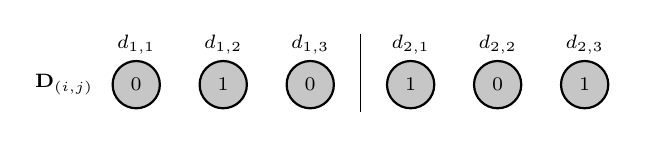
\begin{tikzpicture}[shorten >=1pt,->,draw=black!100, scale=0.85]
	\scriptsize
	\tikzstyle{label}=[text width=3em, text centered]
	\tikzstyle{annot}=[text width=2.5em]
	\tikzstyle{d-node}=[circle,draw=black!100,fill=gray!45,thick,inner sep=0pt,minimum size=6mm]
	
	\def \china{0.6cm}
	\def \data{0cm}
	
	\node[annot] (d-layer) at (0cm,\data) {$\mathbf{D}_{(i,j)}$};
	\draw[-] (4.45cm, \china+1.5mm) -- (4.45cm, \data-4.5mm);
%	\draw[-] (8.55cm, \china+1.5mm) -- (8.55cm, \data-4.5mm);
	%\draw[-] (-1cm, \china+.5cm) -- (13cm, \china+.5cm);
	%\draw[-] (-1cm, \data-.5cm) -- (13cm, \data-.5cm);
	
	\node[label] 	(dl00)	at (1.1cm,\china)		{$d_{1,1}$};
	\node[label] 	(dl01)	at (2.4cm,\china)		{$d_{1,2}$};
	\node[label] 	(dl02)	at (3.7cm,\china)	 	{$d_{1,3}$};
	
	\node[label] 	(dl10)	at (5.2cm,\china) 		{$d_{2,1}$};
	\node[label] 	(dl11) 	at (6.5cm,\china)   	{$d_{2,2}$};
	\node[label] 	(dl12)	at (7.8cm,\china)		{$d_{2,3}$};
	
	% \node[label] 	(dl20) 	at (9.3cm,\china)  		{$d_{3,1}$};
	% \node[label] 	(dl21)	at (10.6cm,\china) 		{$d_{3,2}$};
	% \node[label] 	(dl22) 	at (11.9cm,\china)   	{$d_{3,3}$};
	
	\node[d-node] 	(d00)	at (1.1cm,\data)		{$0$};
	\node[d-node] 	(d01)	at (2.4cm,\data)		{$1$};
	\node[d-node] 	(d02)	at (3.7cm,\data)		{$0$};

	\node[d-node] 	(d10)	at (5.2cm,\data)		{$1$};
	\node[d-node] 	(d11)	at (6.5cm,\data)		{$0$};
	\node[d-node] 	(d12)	at (7.8cm,\data)		{$1$};
	
	% \node[d-node] 	(d20)	at (9.3cm,\data)		{$1$};
	% \node[d-node] 	(d21)	at (10.6cm,\data)		{$1$};
	% \node[d-node] 	(d22)	at (11.9cm,\data)		{$1$};
\end{tikzpicture}
\label{fig:example:subfig0}
}
\end{center}

\usetikzlibrary{positioning}
%\begin{minipage}{.3\textwidth}
\begin{center}
\subfigure[Learning in Progress]{
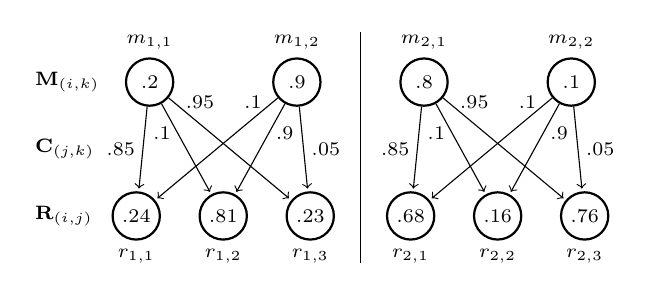
\begin{tikzpicture}[shorten >=1pt,->,draw=black!100, scale=0.85]
	\footnotesize
%	\def \attic{5.95cm}
%	\def \rowtwoht{5.4cm}
%	\def \weightlevel{3.9cm}
%	\def \rowoneht{2.4cm}
%	\def \basement{1.8cm}
%	\def \data{1cm}
%	\def \china{0cm}

	\def \attic{5cm}
	\def \rowtwoht{4.4cm}
	\def \weightlevel{3.4cm}
	\def \rowoneht{2.4cm}
	\def \basement{1.8cm}
	\def \data{1cm}
	\def \china{0cm}
		
	\tikzstyle{m-node}=[circle,draw=black!100,thick,inner sep=0pt,minimum size=6mm]
	\tikzstyle{r-node}=[circle,draw=black!100,thick,inner sep=0pt,minimum size=6mm]
	\tikzstyle{d-node}=[circle,draw=black!100,fill=gray!45,thick,inner sep=0pt,minimum size=6mm]
	%\tikzstyle{dots}=[text width=5ex, text centered]
	\tikzstyle{annot}=[text width=2.5em]
	% labels
	\tikzstyle{label}=[text width=2.5em, text centered]
	\tikzstyle{formula}=[text width=30em, text centered]
	
	\scriptsize
	\node[annot] (hidden-layer) at (0cm,\rowtwoht) {$\mathbf{M}_{(i,k)}$};
	\node[annot] (weights) at (0cm,\weightlevel) {$\mathbf{C}_{(j,k)}$};
	\node[annot] (r-layer) at (0cm,\rowoneht) {$\mathbf{R}_{(i,j)}$};
	
	% hidden layer
	\scriptsize
	\node[m-node] 	(ma00)	at (1.3cm,\rowtwoht)		{$.2$};
	\node[m-node] 	(ma01)	at (3.5cm,\rowtwoht)		{$.9$};
	\node[m-node] 	(ma10)	at (5.4cm,\rowtwoht) 	{$.8$};
	\node[m-node] 	(ma11)	at (7.6cm,\rowtwoht)	 	{$.1$};
	% \node[m-node] 	(m20)	at (9.65cm,\rowtwoht) 	{$.8$};
	% \node[m-node] 	(m21)	at (11.55cm,\rowtwoht)	 	{$.9$};
	
	%\footnotesize
	\node[label]	(ml00) 	at (1.3cm,\attic)		{$m_{1,1}$}; %1.75 -> 1.45
	\node[label]	(ml01) 	at (3.5cm,\attic)		{$m_{1,2}$}; %3.05 -> 3.35
	\node[label] 	(ml10)	at (5.4cm,\attic) 	{$m_{2,1}$};     %5.85 -> 5.55
	\node[label] 	(ml11)	at (7.6cm,\attic)	 	{$m_{2,2}$}; %7.15 -> 7.45
	% \node[label] 	(ml20)	at (9.65cm,\attic) 	{$m_{3,1}$};     %9.95 -> 9.65
	% \node[label] 	(ml21)	at (11.55cm,\attic)	 	{$m_{3,2}$}; %11.25 -> 11.55
	
	\scriptsize
	\node[r-node] 	(ra00)	at (1.1cm,\rowoneht)		{$.24$};
	\node[r-node] 	(ra01)	at (2.4cm,\rowoneht)		{$.81$};
	\node[r-node] 	(ra02)	at (3.7cm,\rowoneht)	 	{$.23$};
	
	\node[r-node] 	(ra10)	at (5.2cm,\rowoneht) 		{$.68$};
	\node[r-node] 	(ra11) 	at (6.5cm,\rowoneht)   	{$.16$};
	\node[r-node] 	(ra12)	at (7.8cm,\rowoneht)		{$.76$};
	
	\node[label] 	(rl00)	at (1.1cm,\basement)		{$r_{1,1}$};
	\node[label] 	(rl01)	at (2.4cm,\basement)		{$r_{1,2}$};
	\node[label] 	(rl02)	at (3.7cm,\basement)	 	{$r_{1,3}$};
	
	\node[label] 	(rl10)	at (5.2cm,\basement) 		{$r_{2,1}$};
	\node[label] 	(rl11) 	at (6.5cm,\basement)   	{$r_{2,2}$};
	\node[label] 	(rl12)	at (7.8cm,\basement)		{$r_{2,3}$};

	\draw[-] (4.45cm, \attic+1.5mm) -- (4.45cm, \basement-1.5mm);

	\scriptsize
	\path
		(ma00)	edge	node [left]	{$.85$} (ra00)
		(ma00)	edge	node [left,xshift=-1mm,yshift=2mm]	{$.1$}	(ra01)
		(ma00)	edge	node [left,xshift=-1mm,yshift=6mm]	{$.95$}	(ra02)

		(ma01)	edge	node [right,xshift=2.5mm,yshift=6mm]	{$.1$}	(ra00)
		(ma01)	edge	node [right,xshift=1mm,yshift=2mm]	{$.9$}	(ra01)
		(ma01)	edge	node [right]	{$.05$} (ra02)
		%
		(ma10)	edge	node [left] {$.85$} (ra10)
		(ma10)	edge	node [left,xshift=-1mm,yshift=2mm]	{$.1$}	(ra11)
		(ma10)	edge	node [left,xshift=-1mm,yshift=6mm] {$.95$}	(ra12)
		
		(ma11)	edge	node [right,xshift=2.5mm,yshift=6mm]	{$.1$}	(ra10)
		(ma11)	edge	node [right,xshift=1mm,yshift=2mm]	{$.9$}	(ra11)
		(ma11)	edge	node [right]	{$.05$} (ra12);
		%
		% (m20)	edge	node [left]	{$.85$}	(r20)
		% (m20)	edge	node [left,xshift=-1mm,yshift=4mm]	{$.1$}	(r21)
		% (m20)	edge	node [left,xshift=-1mm,yshift=10mm]	{$.95$} (r22)
		
		% (m21)	edge	node [right,xshift=3mm,yshift=10mm]		{$.1$}	(r20)
		% (m21)	edge	node [right,xshift=1mm,yshift=4mm]{$.9$}	(r21)
		% (m21)	edge	node [right]	{$.05$}	(r22);		
		
\end{tikzpicture}
\label{fig:example:subfig1}
}
\subfigure[Convergence]{

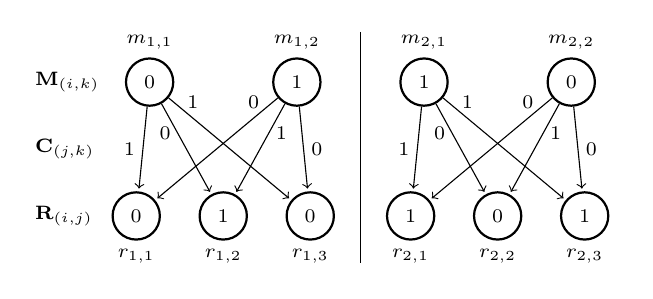
\begin{tikzpicture}[shorten >=1pt,->,draw=black!100, scale=0.85]
	\footnotesize
%	\def \attic{5.95cm}
%	\def \rowtwoht{5.4cm}
%	\def \weightlevel{3.9cm}
%	\def \rowoneht{2.4cm}
%	\def \basement{1.8cm}
%	\def \data{1cm}
%	\def \china{0cm}

%	\def \attic{5.2cm}
%	\def \rowtwoht{4.6cm}
%	\def \weightlevel{3.5cm}
%	\def \rowoneht{2.4cm}
%	\def \basement{1.8cm}
%	\def \data{1cm}
%	\def \china{0cm}

	\def \attic{5cm}
	\def \rowtwoht{4.4cm}
	\def \weightlevel{3.4cm}
	\def \rowoneht{2.4cm}
	\def \basement{1.8cm}
	\def \data{1cm}
	\def \china{0cm}
		
%	\def \attic{5.4cm}
%	\def \rowtwoht{5cm}
%	\def \weightlevel{3.9cm}
%	\def \rowoneht{2.4cm}
%	\def \basement{1.8cm}
%	\def \data{1cm}
%	\def \china{0cm}
	
	\scriptsize
	\tikzstyle{m-node}=[circle,draw=black!100,thick,inner sep=0pt,minimum size=6mm]
	\tikzstyle{r-node}=[circle,draw=black!100,thick,inner sep=0pt,minimum size=6mm]
	\tikzstyle{d-node}=[circle,draw=black!100,fill=gray!45,thick,inner sep=0pt,minimum size=6mm]
	\tikzstyle{annot}=[text width=2.5em]
	% labels
	\tikzstyle{label}=[text width=3em, text centered]
	\tikzstyle{formula}=[text width=30em, text centered]
	\node[annot] (hidden-layer) at (0cm,\rowtwoht) {$\mathbf{M}_{(i,k)}$};
	\node[annot] (weights) at (0cm,\weightlevel) {$\mathbf{C}_{(j,k)}$};
	\node[annot] (r-layer) at (0cm,\rowoneht) {$\mathbf{R}_{(i,j)}$};
	
	\node[m-node] 	(m00)	at (1.3cm,\rowtwoht)		{$0$};
	\node[m-node] 	(m01)	at (3.5cm,\rowtwoht)		{$1$};
	\node[m-node] 	(m10)	at (5.4cm,\rowtwoht) 	{$1$};
	\node[m-node] 	(m11)	at (7.6cm,\rowtwoht)	 	{$0$};
	% \node[m-node] 	(m20)	at (9.65cm,\rowtwoht) 	{$1$};
	% \node[m-node] 	(m21)	at (11.55cm,\rowtwoht)	 	{$1$};
	
	\node[label]	(ml00) 	at (1.3cm,\attic)		{$m_{1,1}$};
	\node[label]	(ml01) 	at (3.5cm,\attic)		{$m_{1,2}$};
	\node[label] 	(ml10)	at (5.4cm,\attic) 	{$m_{2,1}$};
	\node[label] 	(ml11)	at (7.6cm,\attic)	 	{$m_{2,2}$};
	% \node[label] 	(ml20)	at (9.65cm,\attic) 	{$m_{3,1}$};
	% \node[label] 	(ml21)	at (11.55cm,\attic)	 	{$m_{3,2}$};
	
	%\node[m-node] 	(m20)	[right of=m11,xshift=2cm]	 	{$1.0$};
	%\node[m-node] 	(m21)	[right of=m20,xshift=0.5cm]	 	{$1.0$};	
	% reconstructed vector
	\node[r-node] 	(r00)	at (1.1cm,\rowoneht)		{$0$};
	\node[label] 	(rl00)	at (1.1cm,\basement)		{$r_{1,1}$};
	\node[r-node] 	(r01)	at (2.4cm,\rowoneht)		{$1$};
	\node[label] 	(rl01)	at (2.4cm,\basement)		{$r_{1,2}$};
	\node[r-node] 	(r02)	at (3.7cm,\rowoneht)	 	{$0$};
	\node[label] 	(rl02)	at (3.7cm,\basement)	 	{$r_{1,3}$};
	
	\node[r-node] 	(r10)	at (5.2cm,\rowoneht) 		{$1$};
	\node[label] 	(rl10)	at (5.2cm,\basement) 		{$r_{2,1}$};
	\node[r-node] 	(r11) 	at (6.5cm,\rowoneht)   		{$0$};
	\node[label] 	(rl11) 	at (6.5cm,\basement)   		{$r_{2,2}$};
	\node[r-node] 	(r12)	at (7.8cm,\rowoneht)		{$1$};
	\node[label] 	(rl12)	at (7.8cm,\basement)		{$r_{2,3}$};
	
	% \node[r-node] 	(r20) 	at (9.3cm,\rowoneht)  		{$1$};
	% \node[label] 	(rl20) 	at (9.3cm,\basement)  		{$r_{3,1}$};
	% \node[r-node] 	(r21)	at (10.6cm,\rowoneht) 		{$1$};
	% \node[label] 	(rl21)	at (10.6cm,\basement) 		{$r_{3,2}$};
	% \node[r-node] 	(r22) 	at (11.9cm,\rowoneht)   		{$1$};
	% \node[label] 	(rl22) 	at (11.9cm,\basement)   		{$r_{3,3}$};
	
	\draw[-] (4.45cm, \attic+1.5mm) -- (4.45cm, \basement-1.5mm);
%	\draw[-] (8.55cm, \attic+1.5mm) -- (8.55cm, \basement-1.5mm);

	\path
		(m00)	edge	node [left] 	{$1$}	(r00)
		(m00)	edge	node [left,xshift=-1mm,yshift=2mm]	{$0$}	(r01)
		(m00)	edge	node [left,xshift=-3mm,yshift=6mm]	{$1$}	(r02)

		(m01)	edge	node [right,xshift=3mm,yshift=6mm]	{$0$}	(r00)
		(m01)	edge	node [right,xshift=1mm,yshift=2mm]	{$1$}	(r01)
		(m01)	edge	node [right]	{$0$}	(r02)
		%
		(m10)	edge	node [left] 	{$1$}	(r10)
		(m10)	edge	node [left,xshift=-1mm,yshift=2mm]	{$0$}	(r11)
		(m10)	edge	node [left,xshift=-3mm,yshift=6mm] {$1$}	(r12)
		
		(m11)	edge	node [right,xshift=3mm,yshift=6mm]	{$0$}	(r10)
		(m11)	edge	node [right,xshift=1mm,yshift=2mm]	{$1$}	(r11)
		(m11)	edge	node [right]	{$0$}	(r12);
		%
		% (m20)	edge	node [left]	{$1$}	(r20)
		% (m20)	edge	node [left,xshift=-1mm,yshift=4mm]	{$0$}	(r21)
		% (m20)	edge	node [left,xshift=-3mm,yshift=10mm]	{$1$} (r22)
		
		% (m21)	edge	node [right,xshift=3mm,yshift=10mm]		{$0$}	(r20)
		% (m21)	edge	node [right,xshift=1mm,yshift=4mm]{$1$}	(r21)
		% (m21)	edge	node [right]	{$0$}	(r22);		
\end{tikzpicture}
\label{fig:example:subfig2}
}

\begin{framed}
	\centering
	\small
	where
	$\begin{aligned}
	   r_{i,j} = 1 - \Pi_{k=1}^{K} (1 - m_{i,k}c_{j,k}) 
	\end{aligned}$
        \hspace{2em}
        [\textsc{noisy-or} function]
\end{framed}

\end{center}
\caption{A simple MCMM example} % showing learning in progress}
\label{fig:example}
\end{figure}

We can see that while learning is in progress, the cluster activities
($m_{i,k}$) and the cluster centers ($c_{j,k}$) are in flux, as the
error rate is being reduced, but that they converge to values of 0 and
1.  At convergence, a reconstruction node ($r_{i,j}$) is 1 if at least one
$m_{i,k}c_{j,k} = 1$ (and 0 otherwise).

%the activities and the centers are 1 and are 0 otherwise.

% \begin{figure*}[htb]
% \usetikzlibrary{positioning}
% \begin{center}
% \subfigure[Observed Data]{
% \begin{tikzpicture}[shorten >=1pt,->,draw=black!100]
% 	\scriptsize
% 	\tikzstyle{label}=[text width=3em, text centered]
% 	\tikzstyle{annot}=[text width=2.5em]
% 	\tikzstyle{d-node}=[circle,draw=black!100,fill=gray!45,thick,inner sep=0pt,minimum size=6mm]
	
% 	\def \china{0.6cm}
% 	\def \data{0cm}
	
% 	\node[annot] (d-layer) at (0cm,\data) {$\mathbf{D}_{(i,j)}$};
% 	\draw[-] (4.45cm, \china+1.5mm) -- (4.45cm, \data-4.5mm);
% 	\draw[-] (8.55cm, \china+1.5mm) -- (8.55cm, \data-4.5mm);
% 	%\draw[-] (-1cm, \china+.5cm) -- (13cm, \china+.5cm);
% 	%\draw[-] (-1cm, \data-.5cm) -- (13cm, \data-.5cm);
	
% 	\node[label] 	(dl00)	at (1.1cm,\china)		{$d_{1,1}$};
% 	\node[label] 	(dl01)	at (2.4cm,\china)		{$d_{1,2}$};
% 	\node[label] 	(dl02)	at (3.7cm,\china)	 	{$d_{1,3}$};
	
% 	\node[label] 	(dl10)	at (5.2cm,\china) 		{$d_{2,1}$};
% 	\node[label] 	(dl11) 	at (6.5cm,\china)   	{$d_{2,2}$};
% 	\node[label] 	(dl12)	at (7.8cm,\china)		{$d_{2,3}$};
	
% 	\node[label] 	(dl20) 	at (9.3cm,\china)  		{$d_{3,1}$};
% 	\node[label] 	(dl21)	at (10.6cm,\china) 		{$d_{3,2}$};
% 	\node[label] 	(dl22) 	at (11.9cm,\china)   	{$d_{3,3}$};
	
% 	\node[d-node] 	(d00)	at (1.1cm,\data)		{$0$};
% 	\node[d-node] 	(d01)	at (2.4cm,\data)		{$1$};
% 	\node[d-node] 	(d02)	at (3.7cm,\data)		{$0$};

% 	\node[d-node] 	(d10)	at (5.2cm,\data)		{$1$};
% 	\node[d-node] 	(d11)	at (6.5cm,\data)		{$0$};
% 	\node[d-node] 	(d12)	at (7.8cm,\data)		{$1$};
	
% 	\node[d-node] 	(d20)	at (9.3cm,\data)		{$1$};
% 	\node[d-node] 	(d21)	at (10.6cm,\data)		{$1$};
% 	\node[d-node] 	(d22)	at (11.9cm,\data)		{$1$};
% \end{tikzpicture}
% \label{fig:example:subfig0}
% }
% \end{center}

% \usetikzlibrary{positioning}
% %\begin{minipage}{.3\textwidth}
% \begin{center}
% \subfigure[Learning in Progress]{
% \begin{tikzpicture}[shorten >=1pt,->,draw=black!100]
% 	\footnotesize
% 	\def \attic{5.95cm}
% 	\def \rowtwoht{5.4cm}
% 	\def \weightlevel{3.9cm}
% 	\def \rowoneht{2.4cm}
% 	\def \basement{1.8cm}
% 	\def \data{1cm}
% 	\def \china{0cm}
	
% 	\tikzstyle{m-node}=[circle,draw=black!100,thick,inner sep=0pt,minimum size=6mm]
% 	\tikzstyle{r-node}=[circle,draw=black!100,thick,inner sep=0pt,minimum size=6mm]
% 	\tikzstyle{d-node}=[circle,draw=black!100,fill=gray!45,thick,inner sep=0pt,minimum size=6mm]
% 	%\tikzstyle{dots}=[text width=5ex, text centered]
% 	\tikzstyle{annot}=[text width=2.5em]
% 	% labels
% 	\tikzstyle{label}=[text width=3em, text centered]
% 	\tikzstyle{formula}=[text width=30em, text centered]
	
% 	\scriptsize
% 	\node[annot] (hidden-layer) at (0cm,\rowtwoht) {$\mathbf{M}_{(i,k)}$};
% 	\node[annot] (weights) at (0cm,\weightlevel) {$\mathbf{C}_{(j,k)}$};
% 	\node[annot] (r-layer) at (0cm,\rowoneht) {$\mathbf{R}_{(i,j)}$};
	
% 	% hidden layer
% 	\scriptsize
% 	\node[m-node] 	(m00)	at (1.45cm,\rowtwoht)		{$.2$};
% 	\node[m-node] 	(m01)	at (3.35cm,\rowtwoht)		{$.9$};
% 	\node[m-node] 	(m10)	at (5.55cm,\rowtwoht) 	{$.8$};
% 	\node[m-node] 	(m11)	at (7.45cm,\rowtwoht)	 	{$.1$};
% 	\node[m-node] 	(m20)	at (9.65cm,\rowtwoht) 	{$.8$};
% 	\node[m-node] 	(m21)	at (11.55cm,\rowtwoht)	 	{$.9$};
	
% 	%\footnotesize
% 	\node[label]	(ml00) 	at (1.45cm,\attic)		{$m_{1,1}$}; %1.75 -> 1.45
% 	\node[label]	(ml01) 	at (3.35cm,\attic)		{$m_{1,2}$}; %3.05 -> 3.35
% 	\node[label] 	(ml10)	at (5.55cm,\attic) 	{$m_{2,1}$};     %5.85 -> 5.55
% 	\node[label] 	(ml11)	at (7.45cm,\attic)	 	{$m_{2,2}$}; %7.15 -> 7.45
% 	\node[label] 	(ml20)	at (9.65cm,\attic) 	{$m_{3,1}$};     %9.95 -> 9.65
% 	\node[label] 	(ml21)	at (11.55cm,\attic)	 	{$m_{3,2}$}; %11.25 -> 11.55
	
% 	\scriptsize
% 	\node[r-node] 	(r00)	at (1.1cm,\rowoneht)		{$.24$};
% 	\node[r-node] 	(r01)	at (2.4cm,\rowoneht)		{$.81$};
% 	\node[r-node] 	(r02)	at (3.7cm,\rowoneht)	 	{$.23$};
	
% 	\node[r-node] 	(r10)	at (5.2cm,\rowoneht) 		{$.68$};
% 	\node[r-node] 	(r11) 	at (6.5cm,\rowoneht)   	{$.16$};
% 	\node[r-node] 	(r12)	at (7.8cm,\rowoneht)		{$.76$};
	
% 	\node[r-node] 	(r20) 	at (9.3cm,\rowoneht)  		{$.71$};
% 	\node[r-node] 	(r21)	at (10.6cm,\rowoneht) 		{$.83$};
% 	\node[r-node] 	(r22) 	at (11.9cm,\rowoneht)   	{$.77$};
	
% 	\node[label] 	(rl00)	at (1.1cm,\basement)		{$r_{1,1}$};
% 	\node[label] 	(rl01)	at (2.4cm,\basement)		{$r_{1,2}$};
% 	\node[label] 	(rl02)	at (3.7cm,\basement)	 	{$r_{1,3}$};
	
% 	\node[label] 	(rl10)	at (5.2cm,\basement) 		{$r_{2,1}$};
% 	\node[label] 	(rl11) 	at (6.5cm,\basement)   	{$r_{2,2}$};
% 	\node[label] 	(rl12)	at (7.8cm,\basement)		{$r_{2,3}$};
	
% 	\node[label] 	(rl20) 	at (9.3cm,\basement)  		{$r_{3,1}$};
% 	\node[label] 	(rl21)	at (10.6cm,\basement) 		{$r_{3,2}$};
% 	\node[label] 	(rl22) 	at (11.9cm,\basement)   	{$r_{3,3}$};

% 	\draw[-] (4.45cm, \attic+1.5mm) -- (4.45cm, \basement-1.5mm);
% 	\draw[-] (8.55cm, \attic+1.5mm) -- (8.55cm, \basement-1.5mm);

% 	\scriptsize
% 	\path
% 		(m00)	edge	node [left] 	{$.85$}	(r00)
% 		(m00)	edge	node [left,xshift=-1mm,yshift=4mm]	{$.1$}	(r01)
% 		(m00)	edge	node [left,xshift=-1mm,yshift=10mm]	{$.95$}	(r02)

% 		(m01)	edge	node [right,xshift=3mm,yshift=10mm]	{$.1$}	(r00)
% 		(m01)	edge	node [right,xshift=1mm,yshift=4mm]	{$.9$}	(r01)
% 		(m01)	edge	node [right]	{$.05$}	(r02)
% 		%
% 		(m10)	edge	node [left] 	{$.85$}	(r10)
% 		(m10)	edge	node [left,xshift=-1mm,yshift=4mm]	{$.1$}	(r11)
% 		(m10)	edge	node [left,xshift=-1mm,yshift=10mm] {$.95$}	(r12)
		
% 		(m11)	edge	node [right,xshift=3mm,yshift=10mm]	{$.1$}	(r10)
% 		(m11)	edge	node [right,xshift=1mm,yshift=4mm]	{$.9$}	(r11)
% 		(m11)	edge	node [right]	{$.05$}	(r12)
% 		%
% 		(m20)	edge	node [left]	{$.85$}	(r20)
% 		(m20)	edge	node [left,xshift=-1mm,yshift=4mm]	{$.1$}	(r21)
% 		(m20)	edge	node [left,xshift=-1mm,yshift=10mm]	{$.95$} (r22)
		
% 		(m21)	edge	node [right,xshift=3mm,yshift=10mm]		{$.1$}	(r20)
% 		(m21)	edge	node [right,xshift=1mm,yshift=4mm]{$.9$}	(r21)
% 		(m21)	edge	node [right]	{$.05$}	(r22);		
		
% \end{tikzpicture}
% \label{fig:example:subfig1}
% }
% \subfigure[Convergence]{

% \begin{tikzpicture}[shorten >=1pt,->,draw=black!100]
% 	\footnotesize
% 	\def \attic{5.95cm}
% 	\def \rowtwoht{5.4cm}
% 	\def \weightlevel{3.9cm}
% 	\def \rowoneht{2.4cm}
% 	\def \basement{1.8cm}
% 	\def \data{1cm}
% 	\def \china{0cm}
	
% 	\scriptsize
% 	\tikzstyle{m-node}=[circle,draw=black!100,thick,inner sep=0pt,minimum size=6mm]
% 	\tikzstyle{r-node}=[circle,draw=black!100,thick,inner sep=0pt,minimum size=6mm]
% 	\tikzstyle{d-node}=[circle,draw=black!100,fill=gray!45,thick,inner sep=0pt,minimum size=6mm]
% 	\tikzstyle{annot}=[text width=2.5em]
% 	% labels
% 	\tikzstyle{label}=[text width=3em, text centered]
% 	\tikzstyle{formula}=[text width=30em, text centered]
% 	\node[annot] (hidden-layer) at (0cm,\rowtwoht) {$\mathbf{M}_{(i,k)}$};
% 	\node[annot] (weights) at (0cm,\weightlevel) {$\mathbf{C}_{(j,k)}$};
% 	\node[annot] (r-layer) at (0cm,\rowoneht) {$\mathbf{R}_{(i,j)}$};
	
% 	\node[m-node] 	(m00)	at (1.45cm,\rowtwoht)		{$0$};
% 	\node[m-node] 	(m01)	at (3.35cm,\rowtwoht)		{$1$};
% 	\node[m-node] 	(m10)	at (5.55cm,\rowtwoht) 	{$1$};
% 	\node[m-node] 	(m11)	at (7.45cm,\rowtwoht)	 	{$0$};
% 	\node[m-node] 	(m20)	at (9.65cm,\rowtwoht) 	{$1$};
% 	\node[m-node] 	(m21)	at (11.55cm,\rowtwoht)	 	{$1$};
	
% 	\node[label]	(ml00) 	at (1.45cm,\attic)		{$m_{1,1}$};
% 	\node[label]	(ml01) 	at (3.35cm,\attic)		{$m_{1,2}$};
% 	\node[label] 	(ml10)	at (5.55cm,\attic) 	{$m_{2,1}$};
% 	\node[label] 	(ml11)	at (7.45cm,\attic)	 	{$m_{2,2}$};
% 	\node[label] 	(ml20)	at (9.65cm,\attic) 	{$m_{3,1}$};
% 	\node[label] 	(ml21)	at (11.55cm,\attic)	 	{$m_{3,2}$};
	
% 	%\node[m-node] 	(m20)	[right of=m11,xshift=2cm]	 	{$1.0$};
% 	%\node[m-node] 	(m21)	[right of=m20,xshift=0.5cm]	 	{$1.0$};	
% 	% reconstructed vector
% 	\node[r-node] 	(r00)	at (1.1cm,\rowoneht)		{$0$};
% 	\node[label] 	(rl00)	at (1.1cm,\basement)		{$r_{1,1}$};
% 	\node[r-node] 	(r01)	at (2.4cm,\rowoneht)		{$1$};
% 	\node[label] 	(rl01)	at (2.4cm,\basement)		{$r_{1,2}$};
% 	\node[r-node] 	(r02)	at (3.7cm,\rowoneht)	 	{$0$};
% 	\node[label] 	(rl02)	at (3.7cm,\basement)	 	{$r_{1,3}$};
	
% 	\node[r-node] 	(r10)	at (5.2cm,\rowoneht) 		{$1$};
% 	\node[label] 	(rl10)	at (5.2cm,\basement) 		{$r_{2,1}$};
% 	\node[r-node] 	(r11) 	at (6.5cm,\rowoneht)   		{$0$};
% 	\node[label] 	(rl11) 	at (6.5cm,\basement)   		{$r_{2,2}$};
% 	\node[r-node] 	(r12)	at (7.8cm,\rowoneht)		{$1$};
% 	\node[label] 	(rl12)	at (7.8cm,\basement)		{$r_{2,3}$};
	
% 	\node[r-node] 	(r20) 	at (9.3cm,\rowoneht)  		{$1$};
% 	\node[label] 	(rl20) 	at (9.3cm,\basement)  		{$r_{3,1}$};
% 	\node[r-node] 	(r21)	at (10.6cm,\rowoneht) 		{$1$};
% 	\node[label] 	(rl21)	at (10.6cm,\basement) 		{$r_{3,2}$};
% 	\node[r-node] 	(r22) 	at (11.9cm,\rowoneht)   		{$1$};
% 	\node[label] 	(rl22) 	at (11.9cm,\basement)   		{$r_{3,3}$};
	
% 	\draw[-] (4.45cm, \attic+1.5mm) -- (4.45cm, \basement-1.5mm);
% 	\draw[-] (8.55cm, \attic+1.5mm) -- (8.55cm, \basement-1.5mm);

% 	\path
% 		(m00)	edge	node [left] 	{$1$}	(r00)
% 		(m00)	edge	node [left,xshift=-1mm,yshift=4mm]	{$0$}	(r01)
% 		(m00)	edge	node [left,xshift=-3mm,yshift=10mm]	{$1$}	(r02)

% 		(m01)	edge	node [right,xshift=3mm,yshift=10mm]	{$0$}	(r00)
% 		(m01)	edge	node [right,xshift=1mm,yshift=4mm]	{$1$}	(r01)
% 		(m01)	edge	node [right]	{$0$}	(r02)
% 		%
% 		(m10)	edge	node [left] 	{$1$}	(r10)
% 		(m10)	edge	node [left,xshift=-1mm,yshift=4mm]	{$0$}	(r11)
% 		(m10)	edge	node [left,xshift=-3mm,yshift=10mm] {$1$}	(r12)
		
% 		(m11)	edge	node [right,xshift=3mm,yshift=10mm]	{$0$}	(r10)
% 		(m11)	edge	node [right,xshift=1mm,yshift=4mm]	{$1$}	(r11)
% 		(m11)	edge	node [right]	{$0$}	(r12)
% 		%
% 		(m20)	edge	node [left]	{$1$}	(r20)
% 		(m20)	edge	node [left,xshift=-1mm,yshift=4mm]	{$0$}	(r21)
% 		(m20)	edge	node [left,xshift=-3mm,yshift=10mm]	{$1$} (r22)
		
% 		(m21)	edge	node [right,xshift=3mm,yshift=10mm]		{$0$}	(r20)
% 		(m21)	edge	node [right,xshift=1mm,yshift=4mm]{$1$}	(r21)
% 		(m21)	edge	node [right]	{$0$}	(r22);		
% \end{tikzpicture}
% \label{fig:example:subfig2}
% }

% \begin{framed}
% 	\centering
% 	\small
% 	where
% 	$\begin{aligned}
% 	   r_{i,j} = 1 - \Pi_{k=1}^{K} (1 - m_{i,k}c_{j,k}) 
% 	\end{aligned}$
% \end{framed}

% \label{fig:example}
% \caption{MCMM example showing learning in progress}
% \end{center}
% \end{figure*}

